\documentclass[a4paper, openany]{memoir}

\usepackage[utf8]{inputenc}
\usepackage[T1]{fontenc} 
\usepackage[english]{babel}
\usepackage{fancyhdr}
\usepackage{float}
\usepackage{amsmath}
\usepackage{amsthm}
\usepackage{amssymb}
\usepackage[bookmarksopen=true,bookmarksopenlevel=2]{hyperref}
\usepackage{tikz}
\usepackage{indentfirst}

\usepackage{listings}
\usepackage{xcolor}

\pagestyle{fancy}
\fancyhf{}
\fancyhead[LE]{\leftmark}
\fancyhead[RO]{\rightmark}
\fancyhead[RE, LO]{Programming Languages}
\fancyfoot[LE, RO]{\thepage}
\fancyfoot[RE, LO]{Pete Gautam}

\renewcommand{\headrulewidth}{1.5pt}

\usetikzlibrary{shapes}

\definecolor{codegreen}{rgb}{0,0.6,0}
\definecolor{codegray}{rgb}{0.5,0.5,0.5}
\definecolor{codepurple}{rgb}{0.58,0,0.82}
\definecolor{backcolour}{rgb}{0.95,0.95,0.92}

\lstdefinestyle{thestyle}{
    backgroundcolor=\color{backcolour},
    basicstyle=\ttfamily\footnotesize,
    keywordstyle=\color{red!80}\bfseries,
    ndkeywordstyle=\color{blue!80}\bfseries,
    identifierstyle=\color{black},
    commentstyle=\color{codegreen},
    stringstyle=\color{codepurple},
    breakatwhitespace=false,
    breaklines=true,
    captionpos=b,
    keepspaces=true,
    numberstyle=\tiny\color{codegray},
    numbers=left,
    numbersep=2pt,
    showspaces=false,
    showstringspaces=false,
    showtabs=false,          
    tabsize=2
}

\lstdefinelanguage{SVM}{ 
    keywords={LOADC, STOREG, LOADG, JUMPF, JUMP, HALT, CALL, RETURN},
    ndkeywords={COMPLT, COMPGT, ADD, SUB, MUL, DIV},
    sensitive=true,
    comment=[l]{//},
    morecomment=[s]{/*}{*/},
    morestring=[b]',
    morestring=[b]"
}

\lstdefinelanguage{fun}{ 
    keywords={func, while, if, proc, return, read, write},
    ndkeywords={int, char, bool, List, String, Node, Queue, Set, Trie, void, true, false},
    sensitive=true,
    comment=[l]{\#},
    % morecomment=[s]{##}{##},
    morestring=[b]',
    morestring=[b]"
}

\lstdefinelanguage{calc}{ 
    keywords={set, put},
    ndkeywords={},
    sensitive=true,
    comment=[l]{//},
    morecomment=[s]{/*}{*/},
    morestring=[b]',
    morestring=[b]"
}

\lstset{style=thestyle}

\chapterstyle{thatcher}
\setcounter{chapter}{2}

\begin{document}
\chapter{The compilation process}
\section{Syntactic Analysis}
Syntactic analysis checks that the source program is well-formed and determines its phrase structure. The process of syntactic analysis can be broken into 2 further subphrases:
\begin{itemize}
    \item a lexer, which breaks the source program down into tokens; and
    \item a parser, which determines the phrase structure of the program.
\end{itemize}

The syntactic analyser inputs a source program and outputs an AST. Inside the syntactic analyser, the lexer channels a stream of tokens to the parser, as shown below.
\begin{figure}[H]
    \centering
    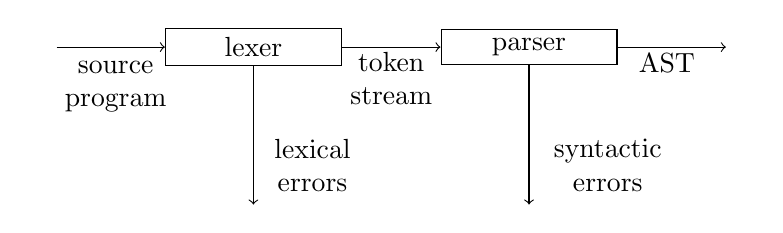
\begin{tikzpicture}
        \node[draw, text width=2cm, align=center] (SA) at (0, 0) {lexer};
        \node[draw, text width=2cm, align=center] (CA) at (3.5, 0) {parser};
        
        \draw[->] (-2.5, 0) -- (SA);
        \node[text width=2cm, align=center] at (-1.75, -.5) {source program};
        \draw[->] (SA) -- (0, -2);
        \node[text width=2cm, align=center] at (0.75, -1.5) {lexical \\ errors};
        
        \draw[->] (SA) -- (CA);
        \node[text width=2cm, align=center] at (1.75, -.4) {token \\ stream};
        \draw[->] (CA) -- (3.5, -2);
        \node[text width=2cm, align=center] at (4.5, -1.5) {syntactic errors};
        
        \node[text width=2cm, align=center] at (5.25, -.2) {AST};
        \draw[->] (CA) -- (6, 0);
    \end{tikzpicture}
    \caption{The data flow within the syntactic analysis phase.}
\end{figure}

\subsection{Tokens}
Tokens are textual symbols that influence the source program's phrase structures, such as literals, identifiers, operators, keywords and punctuation (e.g. commas, colons, parentheses). Each token has a tag and a text. For example, the addition operator might have tag PLUS and text `\texttt{+}'; a numeral might have tag NUM and text `\texttt{1}'; and an identifier might have tag ID and text `\texttt{x}'. These will become the leaves of the AST.

Separators are pieces of text that do not influence the phrase structure, such as spaces and comments. An end-of-line is a separator in most PLs, but a token in Python.

The following are tokens in Calc:
\begin{figure}[H]
    \centering
    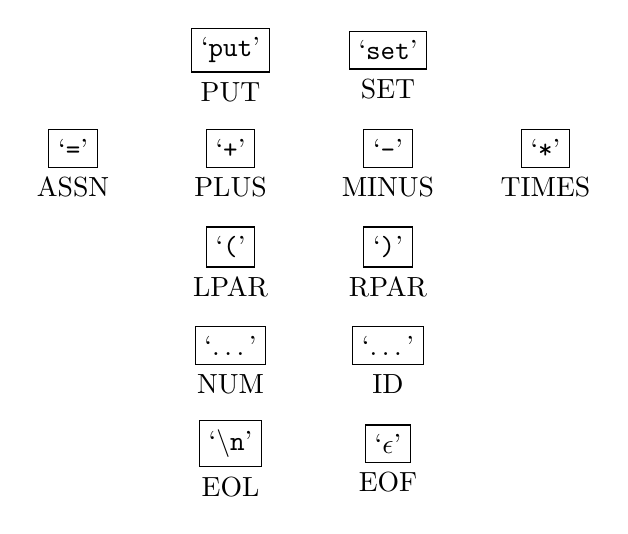
\begin{tikzpicture}
        \node[draw, label=-90:PUT] at (0, 0) {`\texttt{put}'};
        \node[draw, label=-90:SET] at (2, 0) {`\texttt{set}'};
        
        \node[draw, label=-90:ASSN] at (-2, -1.25) {`\texttt{=}'};
        \node[draw, label=-90:PLUS] at (0, -1.25) {`\texttt{+}'};
        \node[draw, label=-90:MINUS] at (2, -1.25) {`\texttt{-}'};
        \node[draw, label=-90:TIMES] at (4, -1.25) {`\texttt{*}'};
        
        \node[draw, label=-90:LPAR] at (0, -2.5) {`\texttt{(}'};
        \node[draw, label=-90:RPAR] at (2, -2.5) {`\texttt{)}'};
        
        \node[draw, label=-90:NUM] at (0, -3.75) {`\dots'};
        \node[draw, label=-90:ID] at (2, -3.75) {`\dots'};
        
        \node[draw, label=-90:EOL] at (0, -5) {`\texttt{\textbackslash n}'};
        \node[draw, label=-90:EOF] at (2, -5) {`$\epsilon$'};
    \end{tikzpicture}
\end{figure}
\noindent Now, assume we have the following Calc program:
\begin{lstlisting}[language=Calc]
set x = 7
put x * (x + 1)
\end{lstlisting}
We get the following token stream from the lexer:
\begin{figure}[H]
    \centering
    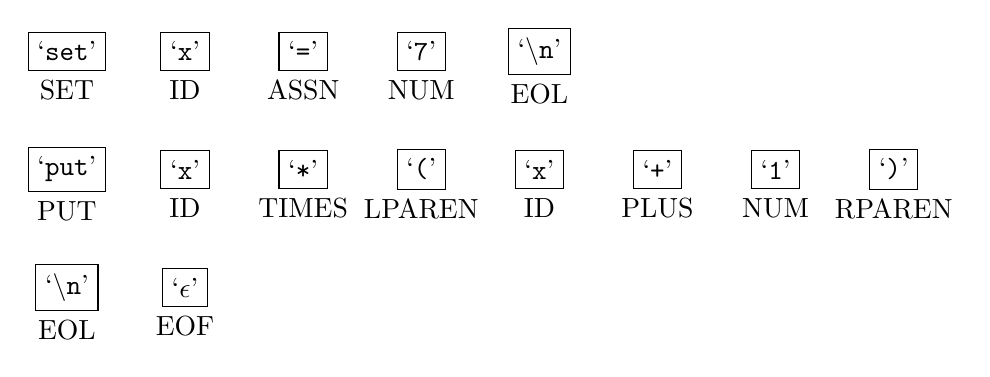
\begin{tikzpicture}
        \node[draw, label=-90:SET] at (0, 0) {`\texttt{set}'};
        \node[draw, label=-90:ID] at (1.5, 0) {`\texttt{x}'};
        \node[draw, label=-90:ASSN] at (3, 0) {`\texttt{=}'};
        \node[draw, label=-90:NUM] at (4.5, 0) {`\texttt{7}'};
        \node[draw, label=-90:EOL] at (6, 0) {`\texttt{\textbackslash n}'};
        
        \node[draw, label=-90:PUT] at (0, -1.5) {`\texttt{put}'};
        \node[draw, label=-90:ID] at (1.5, -1.5) {`\texttt{x}'};
        \node[draw, label=-90:TIMES] at (3, -1.5) {`\texttt{*}'};
        \node[draw, label=-90:LPAREN] at (4.5, -1.5) {`\texttt{(}'};
        \node[draw, label=-90:ID] at (6, -1.5) {`\texttt{x}'};
        \node[draw, label=-90:PLUS] at (7.5, -1.5) {`\texttt{+}'};
        \node[draw, label=-90:NUM] at (9, -1.5) {`\texttt{1}'};
        \node[draw, label=-90:RPAREN] at (10.5, -1.5) {`\texttt{)}'};
        
        \node[draw, label=-90:EOL] at (0, -3) {`\texttt{\textbackslash n}'};
        \node[draw, label=-90:EOF] at (1.5, -3) {`$\epsilon$'};
    \end{tikzpicture}
\end{figure}

The lexer converts source source code into a token stream. At each step, the lexer inspects the next character of the source code and acts accordingly. When there is no source code left, the lexer outputs an EOF token. Depending on the next character, we choose what to do as follows:
\begin{itemize}
    \item space- we discard it
    \item the start of a comment- we scan the rest of the comment and then discard it
    \item punctuation mark- we output the corresponding token
    \item digit- we scan the remaining digits and output the corresponding token (a NUM)
    \item letter- we scan the remaining letters and output the corresponding token (either an ID or a keyword)
\end{itemize}

\subsection{Parser}
The parser converts a token stream into an AST. Parsing is divided into two kinds, reflected in how the parse tree is constructed- top-down (recursive-descent or backtracking), and bottom-up. Recursive-descent (RD) parsing is common and particularly simple. It uses recursive procedures to process the stream of tokens. Give a suitable grammar for the source language, we can systematically write a RD parser for it.

A recursive-descent parser consists of:
\begin{itemize}
    \item a family of parsing methods \texttt{N()}, one for each non-terminal symbol \texttt{N} of the source language's grammar; and
    \item an auxiliary method \texttt{match()}.
\end{itemize}
We say that these methods consume the token stream from left to right. Moreover, in recursive-descent parser, these families of methods perform the following checks/parsing.
\begin{itemize}
    \item The method \texttt{match(t)} checks whether the next token tag \texttt{t}. If yes, it consumes the token. Otherwise, it reports a syntactic error.
    \item For each non-terminal symbol \texttt{N}, the method \texttt{N()} checks whether the next few tokens constitute a phrase of class $N$. If yes, it consumes those tokens (and returns an AST representing the parsed phrase). Otherwise, it reports a syntactic error.
\end{itemize}

Now, we consider a Calc parser. The parsing methods for Calc are:
\begin{itemize}
    \item \texttt{prog()}, which parses a program;
    \item \texttt{com()}, which parses a command;
    \item \texttt{expr()}, which parses an expression;
    \item \texttt{prim()}, which parses an primary expression;
    \item \texttt{var()}, which parses a variable.
\end{itemize}
Assume that we have the following token stream.
\begin{figure}[H]
    \centering
    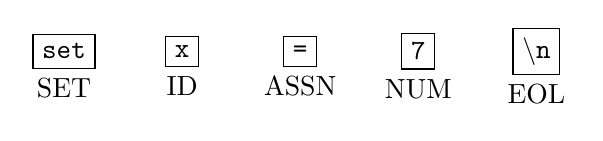
\begin{tikzpicture}
        \node[draw, label=-90:SET] at (0, 0) {\texttt{set}};
        \node[draw, label=-90:ID] at (1.5, 0) {\texttt{x}};
        \node[draw, label=-90:ASSN] at (3, 0) {\texttt{=}};
        \node[draw, label=-90:NUM] at (4.5, 0) {\texttt{7}};
        \node[draw, label=-90:EOL] at (6, 0) {\texttt{\textbackslash n}};
    \end{tikzpicture}
\end{figure}
\noindent Then, the following figure illustrates the recursive nature of the parsing method.
\begin{figure}[H]
    \centering
    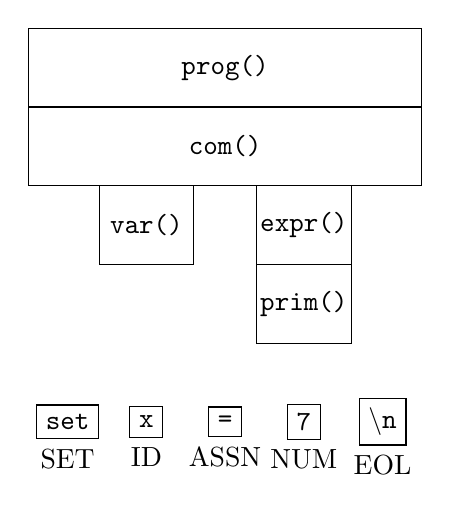
\begin{tikzpicture}
        \draw (0, 0) -- (5, 0) -- (5, -1) -- (0, -1) -- cycle;
        \draw (5, -1) -- (5, -2) -- (0, -2) -- (0, -1);
        \draw (.9, -2) -- (.9, -3) -- (2.1, -3) -- (2.1, -2);
        \draw (2.9, -2) -- (2.9, -3) -- (4.1, -3) -- (4.1, -2);
        \draw (2.9, -3) -- (2.9, -4) -- (4.1, -4) -- (4.1, -3);
        
        \node at (2.5, -.5) {\texttt{prog()}};
        \node at (2.5, -1.5) {\texttt{com()}};
        \node at (1.5, -2.5) {\texttt{var()}};
        \node at (3.5, -2.5) {\texttt{expr()}};
        \node at (3.5, -3.5) {\texttt{prim()}};
        
        \node[draw, label=-90:SET] at (0.5, -5) {\texttt{set}};
        \node[draw, label=-90:ID] at (1.5, -5) {\texttt{x}};
        \node[draw, label=-90:ASSN] at (2.5, -5) {\texttt{=}};
        \node[draw, label=-90:NUM] at (3.5, -5) {\texttt{7}};
        \node[draw, label=-90:EOL] at (4.5, -5) {\texttt{\textbackslash n}};
    \end{tikzpicture}
\end{figure}
% \noindent We say that the entire token stream is consumed by \texttt{com()}, the ID token is consumed by \texttt{var()}, and so on.

In Calc, the EBNF production rule for command is:
\begin{align*}
    \textit{com } =& \text{ `}\texttt{put}\text{'} \textit{ expr eol} \\
    \hspace{2pt} |& \text{ `}\texttt{set}\text{'} \textit{ var } \text{`}\texttt{=}\text{'} \textit{ expr eol}
\end{align*}
So, the parsing method for the command (in Java) is given by the following:
\begin{lstlisting}[language=java]
public void com() {
    // if the next token is `put'
    if (tokenStream.next() == "put") {
        match(PUT);
        expr();
        match(EOL);
    } else if (tokenStream.next() == "set") {
        match(SET);
        var();
        match(ASSN);
        expr();
        match(EOL);
    } else {
        // syntactic error
    }
}
\end{lstlisting}
This is the way we convert EBNF rules into parsing methods. The EBNF production rule for program is:
\[\textit{prog } = \textit{ com}^* \textit{ eof}\]
So, its parsing method is given below.
\begin{lstlisting}[language=java]
public void prog() {
    // while the next token matches a command token,
    while (tokenStream.next().isCom()) {
        com();
    }
    match(EOF);
}
\end{lstlisting}
In general, if we have the rule $N = t$, where $t$ is a terminal system, we produce the following method.
\begin{lstlisting}[language=java]
public void N() {
    match(t);
}
\end{lstlisting}
Instead, if we have the rule $N = M$, where $M$ is a non-terminal system, we produce the following method.
\begin{lstlisting}[language=java]
public void N() {
    M();
}
\end{lstlisting}
If we have the rule $N = RE_1 RE_2$, where $RE_1$ and $RE_2$ are two regular expressions, we produce the following method.
\begin{lstlisting}[language=java]
public void N() {
    // match RE1
    // match RE2
}
\end{lstlisting}
Next, if we have the rule $N = RE^*$, where $RE$ is a regular expression, we produce the following method.
\begin{lstlisting}[language=java]
public void N() {
    // while the next token can be RE,
    while (tokenStream.next().isRE()) {
        // match RE
    }
}
\end{lstlisting}
Now, if we have the rule $N = RE_1 | RE_2$, where $RE_1$ and $RE_2$ are two regular expressions, we produce the following method.
\begin{lstlisting}[language=java]
public void N() {
    // while the next token can be RE1,
    if (tokenStream.next().isRE1()) {
        // match RE1
    }
    // if the next token can be RE2,
    else if (tokenStream.next().isRE2()) {
        // match RE2
    }
    else {
        // syntactic error
    }
}
\end{lstlisting}
This only works if no token can start both $RE_1$ and $RE_2$. In particular, it does not work if a product rule is left-recursive, i.e. it is of the form $N = X | N \ Y$.

Syntactic analysis has a variety of applications.
\begin{itemize}
    \item It is used in compilers, as we have been used to compile Calc.
    \item It is used in XML applications to convert them to tree form.
    \item It is used in web browsers to parse and render HTML documents.
    \item It is used in natural language applications to parse and translate NL documents.
\end{itemize}

\subsection{Compiler generator tools}
A compiler generation tool automates the process of building compiler components. It takes as input the specification of what the compiler component is supposed to do, e.g. the input to a parser generator is a grammar. Examples of compiler generator tools include lex and yacc, JavaCC, ANTLR, etc.

We will look at ANTLR (Another tool for language recognition). It automatically generates a lexer and a recursive-descent parser, starting from a grammar file (.g4). It allows to build and walk a parse tree. We start by expressing the source language's grammar in ANTLR notation, which is very close to the EBNF notation.

ANTLR is composed of two main parts:
\begin{itemize}
    \item the tool, which is used to generate the lexer and the parser, and
    \item the runtime, which is used to run them.
\end{itemize}
The tool is a Java program, even if the runtime is different for every language targeted. When we run ANTLR tool, we can specify the target language (Java by default) to generate a parser, e.g. in Python. ANTLR can generate listeners (by default) and visitors, which are the basis for implementing a contextual analyser and a code generator.

The ANTLR notation is very similar to EBNF. Lexer rules (at the end of the file) are all uppercase, and parser rules are all lowercase. The syntax of a rule is- name, a colon, the definition of the rule, and a terminating semicolon. The Calc grammar in ANTLR is shown below.
\begin{lstlisting}
grammar Calc;
prog
        :   com* EOF
        ;
com
        :   PUT expr EOL            # put
        |   SET var ASSN expr EOL   # set
        ;
expr
        :   prim
            (operator += 
                (PLUS | MINUS | TIMES)
            prim)*                  # op
        ;
prim
        :   NUM                     # num
        |   ID                      # id
        |   LPAR expr RPAR          # parens
        ;
var
        : ID
        ;
PUT     : "put";
SET     : "set";
ASSN    : "=";
PLUS    : "+";
MINUS   : "-";
TIMES   : "*";
LPAR    : "(";
RPAR    : ")"
ID      : "a" .. "z";
NUM     : "0".."9"+;
EOL     : "\r"? "\n";
SPACE   : (" "| "\t")+ -> skip;
\end{lstlisting}
If we run the ANTLR tool on the grammar above, ANTLR will generate the following classes:
\begin{itemize}
    \item The class \texttt{CalcLexer}, which contains methods that convert an input stream (source code) to a token stream.
    \item The class \texttt{CalcParser}, which contains parsing methods \texttt{prog()}, \texttt{com()}, etc. that consume the token stream.
\end{itemize}
We then write a driver program that runs \texttt{CalcParser}'s method \texttt{prog()}:
\begin{lstlisting}[language=java]
public class CalcRun {
    public static void main(String[] args) {
        // create the input stream
        InputStream source = new FileInputStream(args[0]);
        // create the lexer
        CalcLexer lexer = new CalcLexer(
            new ANTLRInputStream(source)
        );
        // run the lexer (creates a token stream)
        CommonTokenStream tokens = new CommonTokenStream(lexer);
        // create a parser
        CalcParser parser = new CalcParser(tokens);
        // run the parser
        ParseTree tree = parser.prog();
    }
}
\end{lstlisting}

When compiled and run, \texttt{CalcRun} performs syntactic analysis on the source program and reports any syntactic errors. It also constructs a syntax tree. The syntax tree can be viewed with the ANTLR \texttt{TestRig} tool. However, \texttt{CalcRun} does not execute the program. The program can be executed by traversing the syntax tree, left to right, depth first, and interpreting each command.

We get the syntax tree automatically by ANTLR. But, to implement an interpreter or compile, we need to walk over the tree and analyse its structure. We will use ASTs to explain, but ANTLR makes use of the full syntax tree with all the tokens. ANTLR uses the Visitor pattern to define tree walkers. It is also possible to use the Listener pattern to do so.

It is possible to configure ANTLR so that we visit the AST. Using a different command, ANTLR generates two further files:
\begin{itemize}
    \item the interface \texttt{CalcVisitor}, which specifies a \texttt{visit} method for each type of syntax tree node, e.g. \texttt{visitProg}, \texttt{visitPut}, etc. The visitor methods have a single parameter \texttt{context}, which has the syntax tree node we are visiting.
    \item the class \texttt{CalcBaseVisitor}, which implements \texttt{CalcVisitor}. Initially, it is formatted to just walk over the syntax tree. We will need to adapt it so that it does what we want it to do.
\end{itemize}

Assume that we want \texttt{CalcRun} to perform calculations, i.e. `\texttt{put}' \textit{expr} should evaluate the expression and print the result, and `\texttt{set}' \textit{var} `\texttt{=}' \textit{expr} should evaluate the expression and then store the result in the given variable. For this, we define the class \texttt{ExecVisitor} that extends \texttt{CalcBaseVisitor} and overrides the \texttt{visit} methods so that they interpret the program while walking over the syntax tree.

The following is the class \texttt{ExecVisitor}:
\begin{lstlisting}[language=java]
class ExecVisitor extends CalcBaseVisitor<Integer> {
    // variables
    int[] store = new int[26];
    
    public Integer visitProg(CalcParser.ProgContext ctx) {
        // interpret every command in the program
        return visitChildren(ctx);
    }
    
    public Integer visitPut(CalcParser.PutContext ctx) {
        // visit the relevant expression
        int value = visit(ctx.expr());
        System.out.println(value);
        // no true value to return
        return 0;
    }
    
    public Integer visitSet(CalcParser.SetContext ctx) {
        // visit the relevant expression
        int value = visit(ctx.expr());
        // get the index corresponding to the variable
        int address = ctx.var().ID().getText().charAt(0) - "a";
        // add the value to the index
        store[address] = value;
        return 0;
    }
    
    public Integer visitOp(CalcParser.OpContext ctx) {
        // get the values and the operations
        List<CalcParser.PrimContext> prims = ctx.prim();
        List<Token> ops = ctx.operator;
        // visit the first value
        int value = visit(prims.get(0));
        // apply the operation to each of the next values
        for (int i = 1; i < prims.size(); i++) {
            switch (ops.get(i-1).getType()) {
                case CalcParser.PLUS;
                    value = value + visit(prims.get(i));
                    break;
                case CalcParser.MINUS;
                    value = value - visit(prims.get(i));
                    break;
                ...
            }
        }
        return value;
    }
    
    public Integer visitNum(CalcParser.NumContext ctx) {
        return Integer.valueOf(ctx.NUM().getText());
    }
    
    public Integer visitId(CalcParser.IdContext ctx) {
        int address = ctx.ID().getText().charAt(0) - "a";
        return store[address];
    }
    
    public Integer visitParens(CalcParser.ParensContext ctx) {
        return visit(ctx.expr());
    }
}
\end{lstlisting}

The driver program needs to be extended to create and call an \texttt{ExecVisitor}.

\begin{lstlisting}[language=java]
public class CalcRun {
    public static void main(String[] args) {
        InputStream source = new FileInputStream(args[0]);
        CalcLexer lexer = new CalcLexer(
            new ANTLRInputStream(source)
        );
        CommonTokenStream tokens = new CommonTokenStream(lexer);
        CalcParser parser = new CalcParser(tokens);
        ParseTree tree = parser.prog();
        ExecVisitor exec = new ExecVisitor();
        exec.visit(tree);
    }
}
\end{lstlisting}
When compiled and run, \texttt{CalcRun} performs syntactic analysis on the source program and then interprets it.

Below is the Fun grammar in the ANTLR notation.
\begin{lstlisting}
grammar Fun;

prog    
        :   var_decl* proc_decl+ EOF        # prog
        ;
var_decl
        :   type ID ASSN expr               # var
        ;
type
        :   BOOL                            # bool
        |   INT
        ;
com
        :   ID ASSN expr                    # assn
        |   WHILE expr COLON seq_com DOT    # while
seq_com
        :   com*                            # seq
        ;
expr    :   e1=sec_expr ...
sec_expr
        :   e1=prim_expr
            ( op = (PLUS | MINUS | TIMES | DIV)
                e2 = sec_expr
            ) ?
prim_expr
        :   NUM                             # num
        |   ID                              # id
        |   LPAR expr RPAR                  # parens
        |   ...
\end{lstlisting}
Running this with the ANTLR tool generates a lexer and a parser. This creates the classes \texttt{FunLexer} and \texttt{FunParser}. The \texttt{prog()} method returns a full syntax tree.
\newpage

\section{Contextual Analysis}
Contextual analysis checks whether the source program (represented by an AST or a syntax tree) satisfies the source language's scope rules and type rules. Logically, there are 2 phases to contextual analysis:
\begin{itemize}
    \item scope checking, which ensures that every identifier used in the source program is declared, and
    \item type checking, which ensures that every operation has operands with the expected types.
\end{itemize}

For example, consider the following source program in Fun:
\begin{lstlisting}[language=fun]
int n = 15
# div program
proc main ():
    while n > 1:
        n = n/2 
    .
.
\end{lstlisting}
\noindent After syntactic analysis, we have the following AST.
\begin{figure}[H]
    \centering
    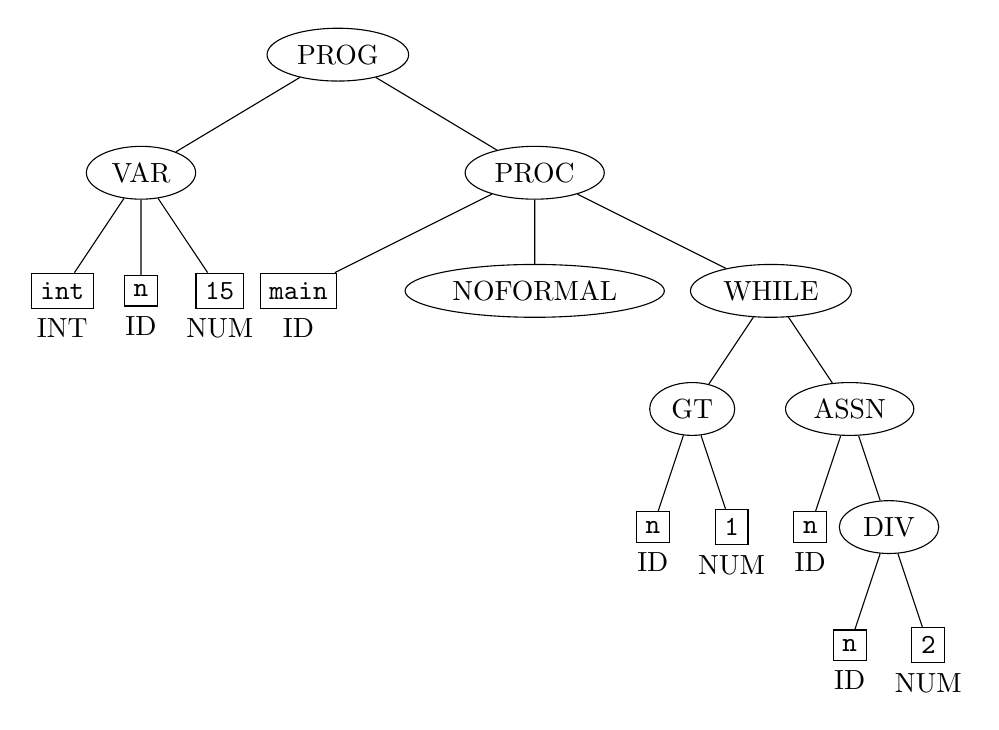
\begin{tikzpicture}[
        level 1/.style={sibling distance=5cm},
        level 2/.style={sibling distance=3cm},
        level 3/.style={sibling distance=2cm},
        level 4/.style={sibling distance=1cm},
    ]
        \node[ellipse, draw] {PROG}
        child[
            level 2/.style={sibling distance=1cm}
        ] {
            node[ellipse, draw] {VAR}
            child {
                node[draw, label=-90:INT] {\texttt{int}}
            }
            child {
                node[draw, label=-90:ID] {\texttt{n}}
            }
            child {
                node[draw, label=-90:NUM] {\texttt{15}}
            }
        }
        child {
            node[ellipse, draw] {PROC}
            child {
                node[draw, label=-90:ID] {\texttt{main}}
            }
            child {
                node[ellipse, draw] {NOFORMAL}
            }
            child {
                node[ellipse, draw] {WHILE}
                child {
                    node[ellipse, draw] {GT}
                    child {
                        node[draw, label=-90:ID] {\texttt{n}}
                    }
                    child {
                        node[draw, label=-90:NUM] {\texttt{1}}
                    }
                }
                child {
                    node[ellipse, draw] {ASSN}
                    child {
                        node[draw, label=-90:ID] {\texttt{n}}
                    }
                    child {
                        node[ellipse, draw] {DIV}
                        child {
                            node[draw, label=-90:ID] {\texttt{n}}
                        }
                        child {
                            node[draw, label=-90:NUM] {\texttt{2}}
                        }
                    }
                }
            }
        };
    \end{tikzpicture}
\end{figure}
\noindent During contextual analysis, we will infer the types of the variables and functions, and get the following enhanced AST:

\begin{figure}[H]
    \centering
    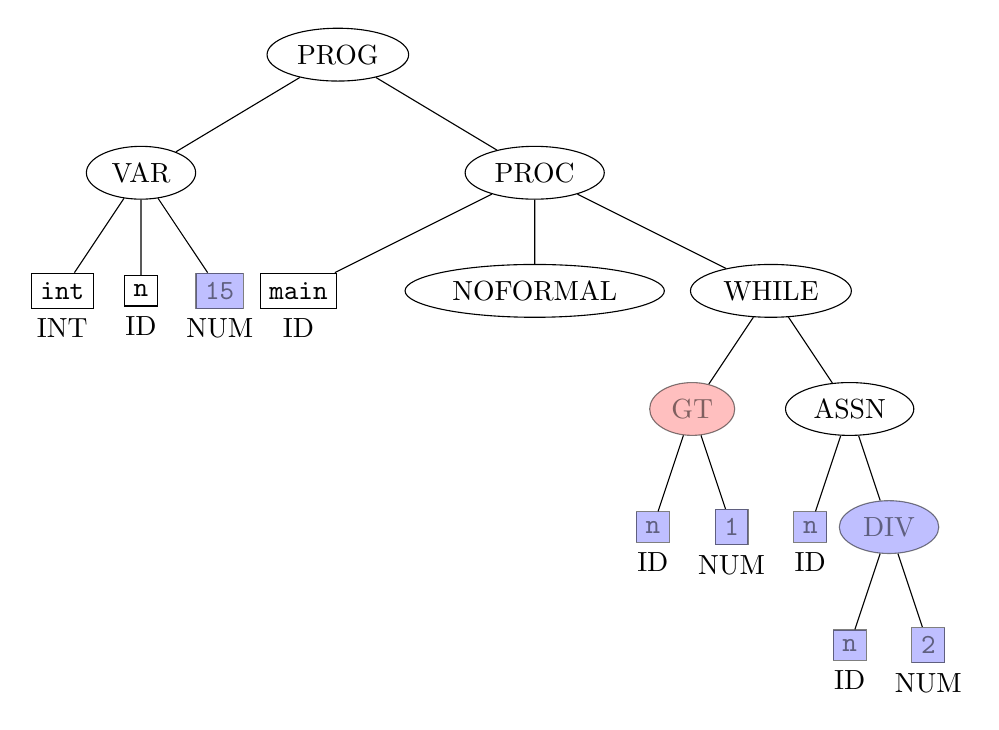
\begin{tikzpicture}[
        level 1/.style={sibling distance=5cm},
        level 2/.style={sibling distance=3cm},
        level 3/.style={sibling distance=2cm},
        level 4/.style={sibling distance=1cm},
    ]
        \node[ellipse, draw] {PROG}
        child[
            level 2/.style={sibling distance=1cm}
        ] {
            node[ellipse, draw] {VAR}
            child {
                node[draw, label=-90:INT] {\texttt{int}}
            }
            child {
                node[draw, label=-90:ID] {\texttt{n}}
            }
            child {
                node[draw, label=-90:NUM, fill=blue!50, opacity=0.5] {\texttt{15}}
            }
        }
        child {
            node[ellipse, draw] {PROC}
            child {
                node[draw, label=-90:ID] {\texttt{main}}
            }
            child {
                node[ellipse, draw] {NOFORMAL}
            }
            child {
                node[ellipse, draw] {WHILE}
                child {
                    node[ellipse, draw, fill=red!50, opacity=0.5] {GT}
                    child {
                        node[draw, label=-90:ID, fill=blue!50, opacity=0.5] {\texttt{n}}
                    }
                    child {
                        node[draw, label=-90:NUM, fill=blue!50, opacity=0.5] {\texttt{1}}
                    }
                }
                child {
                    node[ellipse, draw] {ASSN}
                    child {
                        node[draw, label=-90:ID, fill=blue!50, opacity=0.5] {\texttt{n}}
                    }
                    child {
                        node[ellipse, draw, fill=blue!50, opacity=0.5] {DIV}
                        child {
                            node[draw, label=-90:ID, fill=blue!50, opacity=0.5] {\texttt{n}}
                        }
                        child {
                            node[draw, label=-90:NUM, fill=blue!50, opacity=0.5] {\texttt{2}}
                        }
                    }
                }
            }
        };
    \end{tikzpicture}
\end{figure}
\noindent A red value represents a \texttt{BOOL}, while a blue value represents an \texttt{INT}. We want to keep a type table for each variable. For example, the identifier \texttt{n} is known to be an integer. When we assign \texttt{n = n/2}, this is valid since the division operation returns an integer. In contextual analysis, we check whether the variable exists (scope) and whether it matches the expected type. We also check that the division operator receives 2 integers, and the condition on a while statement is of type \texttt{BOOL}.

\subsection{Scope checking}
Scope checking is the collection and dissemination of information about declared identifiers. The contextual analyser employs a type table. This contains the type of each declared variable, e.g.
\begin{table}[H]
    \centering
    \begin{tabular}{c|c}
        \texttt{n} & \texttt{BOOL} \\
        \hline
        \texttt{fac} & \texttt{INT} $\to$ \texttt{INT} \\
        \texttt{main} & \texttt{VOID} $\to$ \texttt{VOID}
    \end{tabular}
    \caption{A type table}
\end{table}

Whenever an identifier is declared, we put the identifier and its type into the type table. If the identifier is already in the type table (and in the same scope), we report a scope error. Whenever an identifier is used, we check that it is in the type table, and retrieve its type. If the identifier is not in the type table, we report a scope error.

We illustrate the process with Fun scope checking. In Fun, a declaration of a variable identifier is of the form
\[\textit{type id } \texttt{=} \textit{ expr}\]
So, we put the identifier value into the type table, along with its type. If the identifier already exists, we return a scope error.

Similarly, a use of a variable identifier in Fun is of the form
\[\textit{id } \texttt{=} \textit{ expr}\]
In this case, we lookup the identifier in the type type and retrieve its type. If the identifier does not exist, we return a scope error.

\subsection{Type checking}
Type checking is the process of checking that every command and expression is well-typed, meaning that it does not contain any errors. The compiler only performs type checking if the source language is statically typed, i.e. the type of an identifier is known at compile-time.

For example, at each expression, we check the type of each sub-expression. We then infer the type of the expression as a whole. If a sub-expression has unexpected type, we report a type error. Similarly, at each command, we check the type of any constituent expression. If an expression has unexpected type, we report a type error. We do not return a type at the end.

Now, we consider some Fun type checking. The greater than expression is of the form
\[\textit{expr}_1 \text{ `}\texttt{>}\text{' } \textit{expr}_2\]
We walk $\textit{expr}_1$ and check that its type is \texttt{INT}, and do the same thing for $\textit{expr}_2$. We then infer that the type of the whole expression is \texttt{BOOL}. An assignment command is of the form
\[\textit{id } \text{`}\texttt{=}\text{'} \textit{ expr}\]
We lookup the identifier and find its type. We then walk the expression and note its value. At the end, we require that the two types are equivalent. An if-command is of the form
\[\text{`}\texttt{if}\text{' } \textit{expr com}\]
We first walk expression, and check that its type is \texttt{BOOL}. We then walk the command to ensure that there are no type errors within the command.

\subsection{Contextual Analysis in ANTLR}
Contextual analysis is done by walking over the syntax tree. We created a base visitor class during syntactical analysis, so we create another class that extends this class. For contextual analysis, we require also \texttt{SymbolTable}. We use the class \texttt{Type} to representation the type of a value in Fun.

Visting an expression returns the type of the expression, if any. For example, the \texttt{visitNum} method is of the form:
\begin{lstlisting}[language=java]
Type visitNum(FunParser.NumContext ctx) {
    return Type.INT;
}
\end{lstlisting}
The \texttt{visitID} method, that visits an identifier is given below.
\begin{lstlisting}[language=java]
Type visitID(FunParser.IdContext ctx) {
    return retrieve(ctx.ID().getText(), ctx);
}
\end{lstlisting}
To get the type of an identifier, we use the \texttt{retrieve} method. This is returned from the type table. We also pass in the parameter \texttt{ctx} to extract the line number in the case of a type/scope error.

In Fun, an expression is of the form
\[\textit{e}_1 = \textit{ sec\_expr } (\textit{op} = (\text{`}\texttt{=}\text{' } | \text{ `}\texttt{<}\text{' } | \text{ `}\texttt{>}\text{'}) \textit{ e}_2 = \textit{ sec\_expr})^?\]
So, the \texttt{visitExpr} method is the following.
\begin{lstlisting}[language=java]
Type visitExpr(FunParser.ExprContext ctx) {
    Type t1 = visit(ctx.e1);
    if (ctx.e2 != null) {
        Type t2 = visit(ctx.e2);
        return checkBinary(COMPTYPE, t1, t2, ctx);
    }
    else {
        return t1;
    }
}
\end{lstlisting}
\noindent Every expression has $\textit{e}_1$, so we visit it. If $\textit{e}_2$ does not exist, then the type of the expression is the same as the type of $\textit{e}_1$. Otherwise, we visit the second expression and ensure that both the types are \texttt{INT}. The function \texttt{checkBinary} returns the type \texttt{BOOL} after checking the types. The type \texttt{COMPTYPE} is the type representing $\texttt{INT} \times \texttt{INT} \to \texttt{BOOL}$.

In Fun, an assignment command is of the form
\[\textit{ID} \text{ `}\texttt{=}\text{' } \textit{expr}\]
So, the \texttt{visitAssn} method is the following.
\begin{lstlisting}[language=java]
Type visitAssn(FunParser.AssnContext ctx) {
    Type tvar = retrieve(ctx.ID().getText(), ctx);
    Type t = visit(ctx.expr());
    checkType(tvar, t, ctx);
    return null;
}
\end{lstlisting}
We first try to find the type of the identifier. Then, we visit the expression and check that the type of the expression matches the type of the identifier. We return \texttt{null} at the end since a command does not have a type.

In Fun, an if command is of the form
\[\text{`}\texttt{if}\text{' } \textit{expr} \text{ `}\texttt{:}\text{' } \textit{c}_1 = \textit{seq\_com} (\text{`}\texttt{.}\text{' } | \text{ `}\texttt{else:}\text{' } \textit{c}_2 = \textit{seq\_com} \text{ `}\texttt{.}\text{'})\]
So, the \texttt{visitIf} method is the following.
\begin{lstlisting}[language=java]
Type visitIf(FunParser.IfContext ctx) {
    Type t = visit(ctx.expr());
    visit(ctx.c1);
    if (ctx.c2 != null) {
        visit(ctx.c2);
    }
    checkType(Type.BOOL, t, ctx);
    return null;
}
\end{lstlisting}
We first visit the expression, and then the commands. We require the type of the expression to be \texttt{BOOL}.

A sequence of commands is given by
\[\textit{com}^*\]
So, the \texttt{visitSeq} method is the following.
\begin{lstlisting}[language=java]
Type visitSeq(FunParser.SeqContext ctx) {
    visitChildren(ctx);
    return null;
}
\end{lstlisting}
We are just visiting all the children nodes in the tree and not type checking anything at this level.

A variable declaration is given by
\[\textit{type id} \texttt{ = } \textit{expr}.\]
So, the \texttt{visitVar} method is the following.
\begin{lstlisting}[language=java]
Type visitVar(FunParser.VarContext ctx) {
    Type t1 = visit(ctx.type());
    Type t2 = visit(ctx.expr());
    define(ctx.ID().getText(), t1, ctx);
    checkType(t1, t2, ctx);
    return null;
}
\end{lstlisting}
We define the identifier to be of the given type. Then, we check that the type of the expression matches the type of the identifier given.

Finally, a program is given by
\[\textit{var\_decl}^* \textit{proc\_decl}^+ \]
So, the \texttt{visitProg} method is the following.
\begin{lstlisting}[language=java]
Type visitProg(FunParser.ProgContext ctx) {
    predefine();
    visitChildren(ctx);
    Type tmain = retrieve("main", ctx);
    checkType(MAINTYPE, tmain, ctx);
    return null;
}
\end{lstlisting}
The function \texttt{predefine} adds the read and write functions into the type table. We visit all the children to find any type errors within the program. We expect there to be a \texttt{main} procedure in each program, so we check that it exists and its type is $\texttt{VOID} \to \texttt{VOID}$ (called \texttt{MAINTYPE}).

The driver program visits the tree, as given below.
\begin{lstlisting}[language=java]
public static void main(String[] args) {
    ..
    // Syntactic analysis 
    ParseTree tree = parser.program();
    // Contextual analysis
    FunCheckerVisitor checker = new FunCheckVisitor(tokens);
    checker.visit(tree);
}
\end{lstlisting}

\subsection{Representing types}
To implement type checking, we need a way to represent the source language's types. We know that the type of a variable/function can be primitive, Cartesian product, disjoint union or mapping. In the Fun language, we have primitive, Cartesian product and mapping.

We represent Fun primitive data types by \texttt{Type.BOOL} and \texttt{Type.INT} static variables. For a function, we use a mapping type, e.g. $\texttt{T} \to \texttt{T}'$ or $\texttt{VOID} \to \texttt{T}'$. We can represent procedures in a similar way, e.g. $\texttt{T} \to \texttt{VOID}$ or $\texttt{VOID} \to \texttt{VOID}$. We also use mapping types for operators, e.g. \texttt{+}, \texttt{-}, \texttt{*} and \texttt{\textbackslash} are of type $\texttt{(INT} \times \texttt{INT)} \to \texttt{INT}$; \texttt{==}, \texttt{<} and \texttt{>} are of type $(\texttt{INT} \times \texttt{INT)} \to \texttt{BOOL}$; and \texttt{not} is of type $\texttt{BOOL} \to \texttt{BOOL}$.

The class \texttt{Type} is of the following format.
\begin{lstlisting}[language=java]
public abstract class Type {
    public abstract boolean equiv(Type t);
    
    public static class Primitive extends Type {
        ...
    }
    
    public static class Pair extends Type {
        ...
    }
    
    public static class Mapping extends Type {
        ...
    }
}
\end{lstlisting}
The 3 subclasses are used for the 3 types of types. The subclass \texttt{Type.Primitive} has a field that distinguishes different primitive types.
\begin{lstlisting}[language=java]
public static final Type 
    VOID = new Type.Primitive(0),
    BOOL = new Type.Primitive(1),
    INT = new Type.Primitive(2);
\end{lstlisting}
The subclass \texttt{Type.Pair} has two \texttt{Type} fields, which are the types of the pair components, e.g.
\begin{lstlisting}[language=java]
Type prod = new Type.Pair(Type.BOOL, Type.INT);
\end{lstlisting}
represents the type $\texttt{BOOL} \times \texttt{INT}$. Similarly, the subclass \texttt{Type.Mapping} has two \texttt{Type} fields. These are the domain type and range of the mapping type, e.g.
\begin{lstlisting}[language=java]
Type proctype = new Type.Mapping(Type.INT, Type.VOID);
Type optype = new Type.Mapping(
    new Type.Pair(Type.INT, Type.INT), Type.BOOL
);
\end{lstlisting}
The type \texttt{proctype} corresponds to the map $\texttt{INT} \to \texttt{VOID}$, while the type \texttt{optype} corresponds to the map $(\texttt{INT} \times \texttt{INT}) \to \texttt{BOOL}$.

\subsection{Scopes}
In Fun, declarations are global or local. A PL of this structure is said to have flat block structure. The same identifier can be declared both globally and locally, e.g.
\begin{lstlisting}[language=fun]
int x = 1

proc main ():
    int x = 2
    write(x)
.

proc p (bool x):
    if x:
        write(9)
    .
.
\end{lstlisting}
The variable \texttt{x} declared at line 1 is a global variable. The variables \texttt{x} at lines 4 and 9 are local variables, and do not affect the value of the global variable.

The type table must distinguish between global and local entries. The global entries are always present. Local entries are present only when analysing an inner scope. At any given point during analysis of the source program, the same identifier may occur in at most one global entry and at most one local entry. Most PLs have nested scopes instead of this flat global/local scope.

For the Fun program above, the type table of the program at line 1 is the following.
\begin{table}[H]
    \centering
    \begin{tabular}{|c|c|c|}
        \hline
        global & \texttt{x} & \texttt{INT} \\
        \hline
    \end{tabular}
\end{table}
\noindent At line 4, the type table is the following.
\begin{table}[H]
    \centering
    \begin{tabular}{|c|c|c|}
        \hline
        global & \texttt{x} & \texttt{INT} \\
        \hline
        global & \texttt{main} & $\texttt{VOID} \to \texttt{VOID}$ \\
        \hline
        local & \texttt{x} & $\texttt{INT}$ \\
        \hline
    \end{tabular}
\end{table}
\noindent At line 9, the type table is the following.
\begin{table}[H]
    \centering
    \begin{tabular}{|c|c|c|}
        \hline
        global & \texttt{x} & \texttt{INT} \\
        \hline
        global & \texttt{main} & $\texttt{VOID} \to \texttt{VOID}$ \\
        \hline
        global & \texttt{p} & $\texttt{BOOL} \to \texttt{VOID}$ \\
        \hline
        local & \texttt{x} & $\texttt{BOOL}$ \\
        \hline
    \end{tabular}
\end{table}

To implement the type table, we can use 2 hash tables- one for global variables and one for local. This is shown below.
\begin{lstlisting}[language=java]
public class SymbolTable<A> {
    private HashMap<String, A> globals, locals;
    
    public SymbolTable() {
        globals = new HashMap<String, A>();
        locals = null;
    }
}
\end{lstlisting}
When the symbol table gets initialised, the local scope does not exist.

We can enter and leave the local scope whenever we want as follows.
\begin{lstlisting}[language=java]
public void enterLocalScope() {
    locals = new HashMap<String, A>();
}

public void exitLocalScope() {
    locals = null;
}
\end{lstlisting}
So, we are at a local scope if and only if the variable \texttt{locals} is not null.

We can add variables and retrieve them to the symbol table as follows.
\begin{lstlisting}[language=java]
public void put (String id, A attr) {
    if (locals != null) {
        locals.put(id, attr);
    } else {
        globals.put(id, attr);
    }
}

public A get(String id) {
    if (locals != null && locals.containsKey(id)) {
        return locals.get(id);
    } else {
        return globals.get(id);
    }
}
\end{lstlisting}
Each time, we check whether we are in a local scope or a global scope. In the \texttt{put} case, we add the entry to the relevant map. In the \texttt{get} case, we first check whether we have the entry in the local scope. If so, we return that value; otherwise, we return the value at the global scope.

\newpage

\section{Code Generation}
Code generation translates the source program (represented by an AST or a syntax tree) into equivalent object code. In general, code generation can be broken into:
\begin{itemize}
    \item address allocation, where we declare the representation and address of each variable in the source program;
    \item code selection, where we select and generate object code; and
    \item register allocation, where we assign registers to local and temporary variables, if applicable.
\end{itemize}

We will focus on stack-based virtual machines. In that case, address allocation and code generation are straightforward, and we do not have register allocation. For real machines, register allocation is somewhat complicated.

The following is a program in Fun.
\begin{lstlisting}[language=Fun]
int n = 15
proc main():
    while n > 1:
        n = n/2
    .
.
\end{lstlisting}
The corresponding AST for it that we generate after syntactic analysis is given below.
\begin{figure}[H]
    \centering
    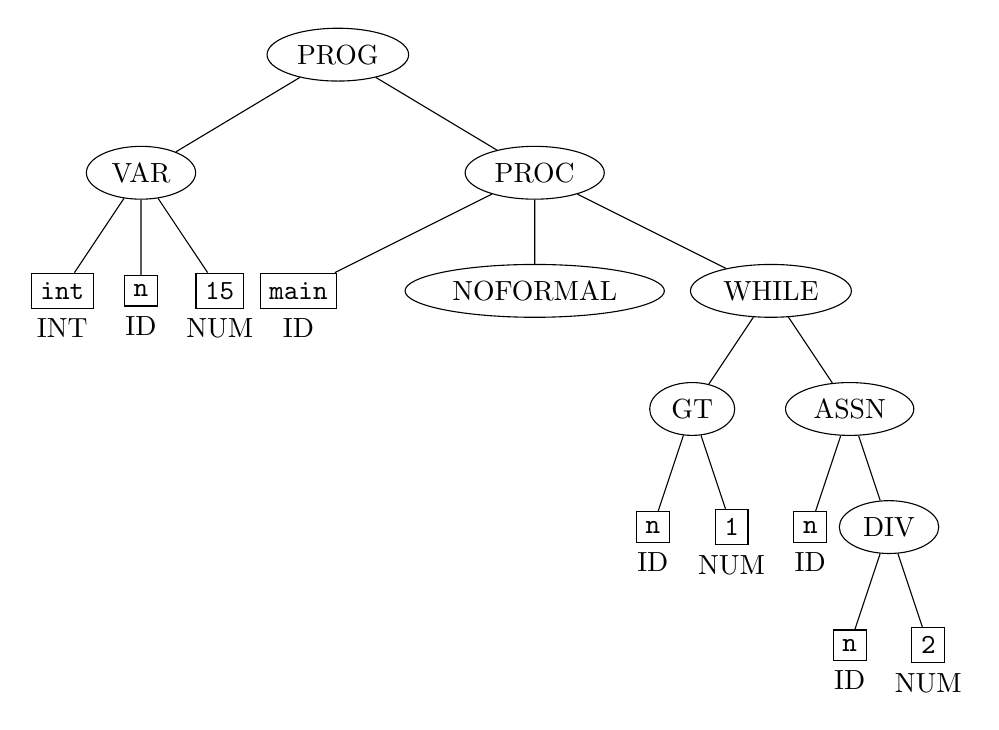
\begin{tikzpicture}[
        level 1/.style={sibling distance=5cm},
        level 2/.style={sibling distance=3cm},
        level 3/.style={sibling distance=2cm},
        level 4/.style={sibling distance=1cm},
    ]
        \node[ellipse, draw] {PROG}
        child[
            level 2/.style={sibling distance=1cm}
        ] {
            node[ellipse, draw] {VAR}
            child {
                node[draw, label=-90:INT] {\texttt{int}}
            }
            child {
                node[draw, label=-90:ID] {\texttt{n}}
            }
            child {
                node[draw, label=-90:NUM] {\texttt{15}}
            }
        }
        child {
            node[ellipse, draw] {PROC}
            child {
                node[draw, label=-90:ID] {\texttt{main}}
            }
            child {
                node[ellipse, draw] {NOFORMAL}
            }
            child {
                node[ellipse, draw] {WHILE}
                child {
                    node[ellipse, draw] {GT}
                    child {
                        node[draw, label=-90:ID] {\texttt{n}}
                    }
                    child {
                        node[draw, label=-90:NUM] {\texttt{1}}
                    }
                }
                child {
                    node[ellipse, draw] {ASSN}
                    child {
                        node[draw, label=-90:ID] {\texttt{n}}
                    }
                    child {
                        node[ellipse, draw] {DIV}
                        child {
                            node[draw, label=-90:ID] {\texttt{n}}
                        }
                        child {
                            node[draw, label=-90:NUM] {\texttt{2}}
                        }
                    }
                }
            }
        };
    \end{tikzpicture}
\end{figure}
\noindent In code generation, we take this AST and convert it into the following SVM object code.
\begin{lstlisting}[language=SVM]
// load constant 15
LOADC 15
// go to 7 = line 8
CALL 7
// stop
HALT
// load the variable at address 0 (variable n)
LOADG 0
// load constant 1
LOADC 1
// compare n > 1
COMPGT
// if false, go to 30 = line 26 (and halt)
JUMPF 30
// load the variable at address 0 (variable n)
LOADG 0
// load constant 2
LOADC 2
// compute n/2
DIV
// store the result at address 0
STOREG 0
// go to 7 = line 8
JUMP 7
// return the value at address 0 (variable n)
RETURN 0
\end{lstlisting}
The address table is:
\begin{table}[H]
    \centering
    \begin{tabular}{|c|c|}
        \hline
        \texttt{n} & 0 (global) \\
        \hline
        \texttt{main} & 7 (code) \\
        \hline
    \end{tabular}
\end{table}

\subsection{Address allocation}
Address allocation requires collection and dissemination of information about declared variables, procedures, etc. The code generator employs an address table. This contains the address of each declared variable, procedure, etc.

At each variable declaration, we allocate a suitable address, and put the identifier and address into address table. Wherever a variable is used (e.g. in a command or expression), we retrieve its address. At each procedure declaration, we note the address of its entry point, and put the identifier and address into the address table. Wherever a procedure is called, we retrieve its address.

We typically allocate consecutive addresses to variables, taking account of their size, e.g. we can have a variable of size 4, 2 or so on. In Fun, all variables are of size 1.

\subsection{Code template}
The code generator will walk the AST. For each construct (e.g. an expression or a command) in the AST, the code generator must emit suitable object code. We must plan what object code will be selected by the code generator.

For each construct in the source language, we devise a code template. This specifies what object code will be selected. The code template to evaluate an expression should include code to evaluate any sub-expressions, together with any other necessary instructions. The code template to execute a command should include code to evaluate any sub-expressions amd code to execute any sub-commands, together with any other necessary instructions.

We will now look at some SVM code templates for different expressions. The addition operation is of the form
\[\textit{expr}_1 \texttt{ + } \textit{expr}_2.\]
The code template here is: 
\begin{itemize}
    \item we evaluate $\textit{expr}_1$; 
    \item we evaluate $\textit{expr}_2$; and 
    \item we run the \texttt{ADD} operation.
\end{itemize}
For example, if we have \texttt{m + (7 * n)}, then the SVM code is:
\begin{lstlisting}[language=SVM]
// load variable m
LOADG 3
// load constant 7
LOADC 7
// load variable n
LOADG 4
// compute 7 * n
MUL
// compute m + (7 * n)
ADD
\end{lstlisting}
Because of the stack nature of data store, this SVM code gets implemented in the expected manner.

The code template specifies what code should be selected. The action specifies what the code generator will actually do to generate the selected code. A template can have several actions, depending on the object code language. For example, the action would be different if we were not using SVM, but the template remains the same.

The assignment command is of the form
\[\textit{ID} \texttt{ = } \textit{expr}\]
The code template here is:
\begin{itemize}
    \item we evaluate \textit{expr}
    \item we run the \texttt{STOREG} or \texttt{STOREL} operation to store the value at a specified address offset.
\end{itemize}
For example, if we have \texttt{m = n - 9}, then the SVM code is:
\begin{lstlisting}[language=SVM]
// load the variable n
LOADG 4
// load the constant 9
LOADC 9
// compute n - 9
SUB
// store the result as variable m
STOREG 3
\end{lstlisting}
The code generator action for the assignment command is:
\begin{itemize}
    \item walk \texttt{expr} and generate the code;
    \item lookup the identifier and retrieve its address $d$;
    \item emit instruction \texttt{STOREG} $d$ (if global variable), or \texttt{STOREL} $d$ (if local variable).
\end{itemize}

The code generator emits instructions one by one. When an instruction is emitted, it is added to the end of the object code. At the destination of a jump instruction, the code generator must note the destination address and incorporate it into the jump instruction.

For a backward jump, the destination address is already known when the jump instruction is emitted. On the other hand, for a forward jump, the destination address is unknown when the jump instruction is emitted. In that case, we emit an incomplete jump address (with 0 in its address field) and note its address. When the destination address becomes known later, we patch that address into the jump instruction.

We can see this in the if command. An if command is of the form
\[\texttt{if } \textit{expr } \textit{com}\]
The code template is:
\begin{itemize}
    \item evaluate the \textit{expr}
    \item \texttt{JUMPF} to the end of \textit{com}
    \item evaluate the \textit{com}
    \item patch the location of \texttt{JUMPF} with the end of \textit{com} evaluation.
\end{itemize}
For example, if we want to execute \texttt{if m > n: m = n.}, then we get the following SVM code:
\begin{lstlisting}[language=SVM]
// load variable m
LOADG 3
// load variable n
LOADG 4
// compute m > n
COMPGT
// if false, jump to the end
JUMPF *
// load variable m
LOADG 4
// store as variable n
STOREG 3
\end{lstlisting}
The code generator action for if-command is:
\begin{itemize}
    \item walk \textit{expr} and generate code;
    \item emit the instruction \texttt{JUMPF 0};
    \item walk \textit{com} and generate code;
    \item patch the correct address into the \texttt{JUMPF} instruction.
\end{itemize}

Next, we consider the while command. It is of the form
\[\texttt{while} \textit{ expr com}\]
The code template here is:
\begin{itemize}
    \item evaluate the \textit{expr}
    \item \texttt{JUMPF} to after the end of \textit{com}
    \item evaluate the \textit{com}
    \item \texttt{JUMP} to before \textit{expr}
\end{itemize}

\subsection{Code generation with ANTLR}
The code generator is a visitor, with a similar structure to the contextual analysis visitor. For each type of syntax tree node, the visit method implements the code generation action. The preamble is given below:
\begin{lstlisting}[language=java]
// creates an instance of SVM. The code generator will emit
// instructions directly into its code store
SVM obj = new SVM();
int globalvaraddr = 0;
int localvaraddr = 0;
int currentLocale = Adress.GLOBAL;

SymbolTable<Address> addrTable = new SymbolTable<>();
\end{lstlisting}

We need to implement visit methods for each kind of node in the AST. The following is the method for visiting numbers.
\begin{lstlisting}[language=java]
void visitNum(FunParser.NumContext ctx) {
    int value = Integer.parseInt(ctx.NUM().getText());
    obj.emit12(SVM.LOADC, value);
}
\end{lstlisting}
The command \texttt{emit12} means 1 opcode and 2 byte operand. 

The visit identifier method is given below.
\begin{lstlisting}[language=java]
void visitId(FunParser.IDContext ctx) {
    String id = ctx.ID().getText();
    Address varaddr = addrTable.get(id);
    switch (varaddr.locale) {
        case Address.GLOBAL:
            obj.emit12(SVM.LOADG, varaddr.offset);
            break;
        case Address.LOCAL:
            obj.emit12(SVM.LOADL, varaddr.offset);
            break;
    }
}
\end{lstlisting}

The visit expression method is given below.
\begin{lstlisting}[language=java]
void visitExpr(FunParser.ExprContext ctx) {
    // generate code to evaluate e1
    visit(ctx.e1);
    // if e2 exists, then generate code to evaluate e2
    if (ctx.e2 != null) {
        visit(ctx.e2);
        
        // generate an instruction for each operator
        switch (ctx.op.getType()) {
            case FunParser.EQ:
                obj.emit1(SVM.CMPEQ);
                break;
            case FunParser.LT:
                obj.emit1(SVM.CMPLT);
                break;
            case FunParser.GT:
                obj.emit1(SVM.CMPGT);
                break;
        }
    }
}
\end{lstlisting}
The command \texttt{emit1} means just 1 opcode.

The visit assignment method is given below.
\begin{lstlisting}[language=java]
void visitAssn(FunParser.AssnContext ctx) {
    // generate code to evaluate expr
    visit(ctx.expr());
    String id = ctx.ID().getText();
    
    // find the address of the variable
    // this always succeeds, because we added the address
    // during contextual analysis
    Address varaddr = addrTable.get(id);
    switch (varaddr.locale) {
        case Address.GLOBAL:
            obj.emit12(SVM.STOREG, varaddr.offset);
            break;
        case Address.LOCAL:
            obj.emit12(SVM.STOREL, varaddr.offset);
            break;

    }
}
\end{lstlisting}

The visit if method is given below.
\begin{lstlisting}[language=java]
void visitIf(Funparser.IfContext ctx) {
    visit(ctx.expr());
    int condaddr = obj.currentOffset();
    // This has to be patched later
    obj.emit12(SVM.JUMPF, 0);
    // IF without ELSE
    if (ctx.c2 == null) {
        visit(ctx.c1);
        int exitaddr = obj.currentOffset();
        obj.patch12(condaddr, exitaddr);
    } else {
        visit(ctx.c1);
        int jumpaddr = obj.currentOffset();
        obj.emit12(SVM.JUMP, 0);
        int elseaddr = obj.currentOffset();
        obj.patch12(conaddr, elseaddr);
        visit(ctx.c2);
        int exitaddr = obj.currentOffset();
        obj.patch12(jumpaddr, exitaddr);
    }
}
\end{lstlisting}

The visit var method is given below.
\begin{lstlisting}[language=java]
void visitVar(FunParser.VarContext ctx) {
    visit(ctx.expr());
    String id = ctx.ID().getText();
    switch (currentLocale) {
        // adding the variable to the address table always 
        // succeeds because we have done contextual analysis
        case Address.LOCAL:
            addrTable.put(id, new Address(localvaraddr++, 
                Address.LOCAL));
            break;
        case Address.GLOBAL:
            addrTable.put(id, new Address(globalvaraddr++, 
                Address.GLOBAL));
            break;
    }
}
\end{lstlisting}

\subsection{Storage organisation}
Each variable occupies storage space throughout its lifetime. This storage must be allocated at the start of the variable's lifetime and deallocated at the end of the variable's lifetime. For a statically typed PL, every variable's type is known to the compiler. Moreover, we assume that all variables of the same type occupy the same amount of storage space.

A global variable's lifetime is the program's entire runtime. For global variables, the compiler allocates fixed storage space. On the other hand, a local variable's lifetime is an activation of the block in which variable is declared. The lifetime of local variables are nested. For local variables, the compiler allocates storage space on a stack.

At any given time, the stack contains one or more activation frames. The frame at the base of the stack contains the global variables. For each active procedure $P$, there is a frame containing $P$'s local variables. An active procedure is one that has been called but not yet returned. A frame for a procedure $P$ is pushed onto the stack when $P$ is called, and popped off the stack when $P$ returns.

The compiler fixes the size and layout of each frame. The offset of each global and local variable (relative to the frame) is known to the compiler.

This can be seen in the figure below.
\begin{figure}[H]
    \centering
    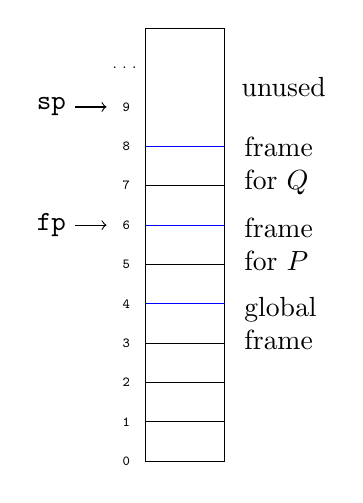
\begin{tikzpicture}
        \draw (0, 0) -- (1, 0)
            -- (1, 5.5)
            -- (0, 5.5)
            -- cycle;
        
        \foreach \i in {0, 1, ..., 8} {
            \node at (-0.25, \i*0.5) {\tiny\texttt{\i}};
            \draw (0, \i*0.5) -- (1, \i*0.5);
        }
        \draw[blue] (0, 2) -- (1, 2);
        \draw[blue] (0, 3) -- (1, 3);
        \draw[blue] (0, 4) -- (1, 4);
        
        \node at (-0.25, 4.5) {\tiny\texttt{9}};
        \node at (-0.25, 5) {\tiny$\dots$};
        
        \node[text width=1cm] at (1.75, 1.75) {global frame};
        \node[text width=1cm] at (1.75, 2.75) {frame for $P$};
        \node[text width=1cm] at (1.75, 3.75) {frame for $Q$};
        \node at (1.75, 4.75) {unused};
        
        \draw[->] (-.9, 4.5) -- (-.5, 4.5);
        \node at (-1.2, 4.5) {\texttt{sp}};
        
        \draw[->] (-.9, 3) -- (-.5, 3);
        \node at (-1.2, 3) {\texttt{fp}};
    \end{tikzpicture}
\end{figure}
\noindent The diagram represents the SVM data store when the main program has called $P$, and $P$ has called $Q$. A local frame contains the local variables, the return address and the dynamic link which points to the previous frame. The stack pointer (sp) points to the first cell above the top of the stack, and the frame pointer (fp) points to the first cell of the topmost frame.

% TODO: Compilation of a program

We will use this for procedure declaration, whose visit method is given below.
\begin{lstlisting}[language=java]
void visitProc(FunParser.ProcContext ctx) {
    String id = ctx.ID().getText();
    Address procaddr = new Address(obj.currentOffset(), 
        Address.CODE);
    addrTable.put(id, procaddr);
    addrTable.enterLocalScope();
    currentLocale = Address.LOCAL;
    localvaraddr = 2;
    
    FunParser.Formal_declContext fd = ctx.formal_decl();
    if (fd != null)
        visit(fd);
    List<FunParser.Var_declContext> var_decl = ctx.var_decl();
    for (FunParser.Var_declContext vd : var_decl) {
        visit(vd);
    }
    visit(ctx.seq_com());
    // 0 because there is no result
    obj.emit11(SVM.RETURN, 0);
    addrTable.exitLocalScope();
    currentLocale = Address.GLOBAL;
}
\end{lstlisting}

The visit formal method is given below.
\begin{lstlisting}[language=java]
void visitFormal(FunParser.FormalContext ctx) {
    FunParser.TypeContext tc = ctx.type();
    if (tc != null) {
        String id = ctx.ID().getText();
        // A parameter is like a local variable
        addrTable.put(id, new Address(localvaraddr++, 
            Address.LOCAL));
        // copy arguments into the stack frame
        obj.emit11(SVM.COPYARG, 1);
    }
}
\end{lstlisting}

Finally, the visit program method is given below.
\begin{lstlisting}[language=java]
void visitProg(FunParser.ProgContext ctx) {
    // add read and write to the address table
    predefine();
    List<FunParser.Var_declContext> var_decl = ctx.var_decl();
    for (FunParser.Var_declContext vd: var_decl) {
        visit(vd);
    }
    int calladdr = obj.currentOffset();
    // call the main method (will patch)
    obj.emit12(SVM.CALL, 0);
    obj.emit1(SVM.HALT);
    List<FunParser.Proc_declContext> proc_decl = ctx.proc_decl();
    for (FunParser.Proc_declContext pd : proc_decl) {
        visit(pd);
    }
    int mainaddr = addrTable.get("main").offset;
    obj.patch12(calladdr, mainaddr);
}
\end{lstlisting}

The code generator must distinguish between three kinds of addresses:
\begin{itemize}
    \item code addresses, which refers to an instruction within the space allocated to the object code.
    \item global address, which refers to a location within the space allocated to global variables.
    \item local address, which refers to a location within a space allocated to a group of local variables.
\end{itemize}

The implementation of address in Java is given below.
\begin{lstlisting}[language=java]
public class Address {
    public static final int 
        CODE = 0, GLOBAL = 1, LOCAL = 2
    public int offset;
    // CODE, GLOBAL or LOCAL
    public int locale; 
    
    public Address(int off, int loc) {
        offset = off; 
        locale = loc;
    }
}
\end{lstlisting}
\newpage

\section{Runtime organisation}
% TODO: First slide

The representation of each primitive type may be language defined or implementation defined. Typically, this is a fixed amount of bits. Some primitive types include \texttt{BOOL}, \texttt{CHAR}, \texttt{INT} and \texttt{FLOAT}.

We represent an array by juxtaposing its components. The following is a representation of an array of type $\{0, 1, 2 \dots\} \to T$.
\begin{figure}[H]
    \centering
    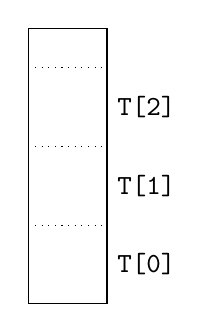
\begin{tikzpicture}
        \draw (0, 0) rectangle (1, 3.5);

        \draw[dotted] (0, 1) -- (1, 1);
        \node at (1.5, 0.5) {\texttt{T[0]}};

        \draw[dotted] (0, 2) -- (1, 2);
        \node at (1.5, 1.5) {\texttt{T[1]}};
        
        \draw[dotted] (0, 3) -- (1, 3);
        \node at (1.5, 2.5) {\texttt{T[2]}};
    \end{tikzpicture}
\end{figure}
\noindent The offset of \texttt{T[i]} from the base. If each element is of 4 bits, then \texttt{T[0]} is at offset 0; \texttt{T[1]} is at offset 4; etc.

Each component takes the same size. The offset of array component $i$ (relative to the array's base address) is linearly related to $i$, i.e.
\[\text{offset} = \text{size of component} \times i.\]
Since $i$ is not known to the compiler, the offset of component $i$ gets calculated at runtime.

We represent a tuple by juxtaposing its components in a similar way. For example, the representation of tuples of type $T_1 \times T_2 \times \dots T_n$ is given below.
\begin{figure}[H]
    \centering
    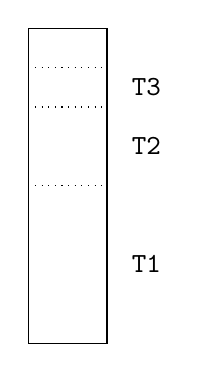
\begin{tikzpicture}
        \draw (0, 0) rectangle (1, 4);

        \draw[dotted] (0, 2) -- (1, 2);
        \node at (1.5, 1) {\texttt{T1}};

        \draw[dotted] (0, 3) -- (1, 3);
        \node at (1.5, 2.5) {\texttt{T2}};

        \draw[dotted] (0, 3.5) -- (1, 3.5);
        \node at (1.5, 3.25) {\texttt{T3}};
    \end{tikzpicture}
\end{figure}
\noindent The components need not be of the same type and can have different sizes, as shown above. The compiler can easily compute the offset. For example, the offset of component 1 is 0, and the offset of component 2 is the size of \texttt{T1}, and so on. 

An object is a tagged tuple. So, we represent an object by juxtaposing its components (i.e. instance variables) with a class tag. Assume that we have a class $C$ with instance variables of types $T_1, \dots, T_n$. The following is the representation of an object of class $C$.
\begin{figure}[H]
    \centering
    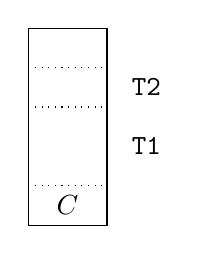
\begin{tikzpicture}
        \draw (0, 0) rectangle (1, 2.5);

        \draw[dotted] (0, 0.5) -- (1, 0.5);
        \node at (0.5, 0.25) {$C$};

        \draw[dotted] (0, 1.5) -- (1, 1.5);
        \node at (1.5, 1) {\texttt{T1}};

        \draw[dotted] (0, 2) -- (1, 2);
        \node at (1.5, 1.75) {\texttt{T2}};
    \end{tikzpicture}
\end{figure}
\noindent We have the class tag at the bottom, followed by the instance variable components. The compiler knows the size of each component, so the memory can be allocated at compile-time.

Next, consider we have a class $C'$ that is a subclass of $C$, with additional instance variables $T_1', \dots, T_m'$. The following is the representation of an object of class $C'$.
\begin{figure}[H]
    \centering
    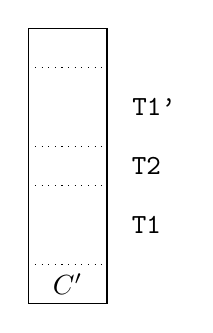
\begin{tikzpicture}
        \draw (0, 0) rectangle (1, 3.5);

        \draw[dotted] (0, 0.5) -- (1, 0.5);
        \node at (0.5, 0.25) {$C'$};

        \draw[dotted] (0, 1.5) -- (1, 1.5);
        \node at (1.5, 1) {\texttt{T1}};

        \draw[dotted] (0, 2) -- (1, 2);
        \node at (1.5, 1.75) {\texttt{T2}};

        \draw[dotted] (0, 3) -- (1, 3);
        \node at (1.6, 2.5) {\texttt{T1'}};
    \end{tikzpicture}
\end{figure}
\noindent We use the class tag $C'$ instead of $C$ here. This allows for dynamic dispatch.

\subsection{Storage organisation}
Each variable occupies storage space throughout its lifetime. That storage space must be allocated at the start of the lifetime and deallocated at the end of the lifetime. We assume that the PL is statically typed, and that all variables of the same type occupy the same amount of storage space.

A global variable's lifetime is the program's entire runtime. So, the compiler allocates fixed storage space for them. A local variable's lifetime is an activation of the block in which the variable is declared. The lifetime of local variables are nested. So, the compiler allocates storage space on a stack.

At any given time, the stack contains one or more activation frames. An active procedure is one that has been called but not yet returned. The frame at the base of the stack contains the global variables. For each active procedure $P$, there is a frame containing $P$'s local variables. A frame for procedure $P$ is pushed onto the stack when $P$ is called, and popped off the stack when $P$ returns.

The compiler fixes the size and the layout of each frame. The offset of each global and local variable (relative to the base of the frame) is known to the compiler.

% The following figure shows the SVM data store when the main program has called $P$, and $P$ has called $Q$. The stack pointer \texttt{sp} points to the first free cell above the top of the stack. The frame pointer \texttt{fp} points to the first cell of the topmost frame.
% TODO: SVM has been done above as well

A heap variable's lifetime starts when the heap variable is created. It ends when it is destroyed or becomes unreachable. The lifetimes of heap variables follow no pattern. Heap variables occupy a storage region called the heap. 

At any given time, the heap contains all currently-live heap variables, interspersed with free space. When a new heap variable is created, some free space is allocated to it. When a heap variable is destroyed, its allocated space reverts to being free.

A PL's runtime system typically includes the heap manager. It keeps track of free space within the heap. It is usually done by a free-list. This is a linked list of free areas of various sizes. The heap manager provides a routine to create and destroy a heap variable.

We illustrate this with an example. Assume that we start with the following state of local and heap variables.
\begin{figure}[H]
    \centering
    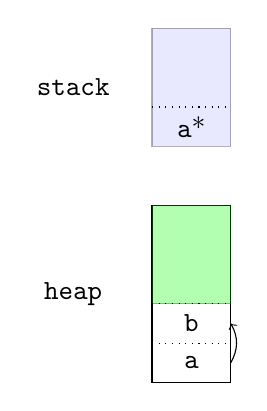
\begin{tikzpicture}
        \draw (0, 0) rectangle (1, 2.25);
        \draw[fill=green, opacity=0.3] (0, 1) rectangle (1, 2.25);
        
        \draw[dotted] (0, 0.5) -- (1, 0.5);
        \node at (0.5, 0.25) {\texttt{a}};

        \draw[dotted] (0, 1) -- (1, 1);
        \node at (0.5, 0.75) {\texttt{b}};

        \draw (1, 0.25) edge[->, bend right] (1, 0.75);

        \draw[fill=blue!30, opacity=0.3] (0, 3) rectangle (1, 4.5);

        \draw[dotted] (0, 3.5) -- (1, 3.5);
        \node at (0.5, 3.25) {\texttt{a}*};

        \node at (-1, 1.125) {\texttt{heap}};
        \node at (-1, 3.75) {\texttt{stack}};
    \end{tikzpicture}
\end{figure}
\noindent The green section within the heap is all the free space we have. We now allocate the variable \texttt{c}. It gets added to both the heap and the stack since we have a pointer to \texttt{c} in code.
\begin{figure}[H]
    \centering
    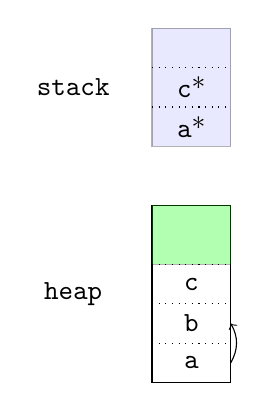
\begin{tikzpicture}
        \draw (0, 0) rectangle (1, 2.25);
        \draw[fill=green, opacity=0.3] (0, 1.5) rectangle (1, 2.25);
        
        \draw[dotted] (0, 0.5) -- (1, 0.5);
        \node at (0.5, 0.25) {\texttt{a}};

        \draw[dotted] (0, 1) -- (1, 1);
        \node at (0.5, 0.75) {\texttt{b}};
        
        \draw[dotted] (0, 1.5) -- (1, 1.5);
        \node at (0.5, 1.25) {\texttt{c}};

        \draw (1, 0.25) edge[->, bend right] (1, 0.75);

        \draw[fill=blue!30, opacity=0.3] (0, 3) rectangle (1, 4.5);

        \draw[dotted] (0, 3.5) -- (1, 3.5);
        \node at (0.5, 3.25) {\texttt{a}*};
        
        \draw[dotted] (0, 4) -- (1, 4);
        \node at (0.5, 3.75) {\texttt{c}*};

        \node at (-1, 1.125) {\texttt{heap}};
        \node at (-1, 3.75) {\texttt{stack}};
    \end{tikzpicture}
\end{figure}
\noindent Now, we change \texttt{a.next} from \texttt{b} to \texttt{c}.
\begin{figure}[H]
    \centering
    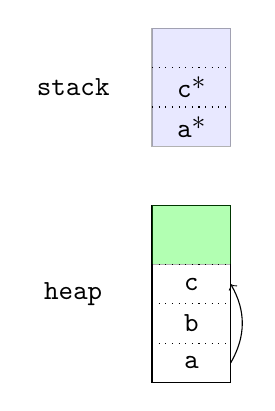
\begin{tikzpicture}
        \draw (0, 0) rectangle (1, 2.25);
        \draw[fill=green, opacity=0.3] (0, 1.5) rectangle (1, 2.25);
        
        \draw[dotted] (0, 0.5) -- (1, 0.5);
        \node at (0.5, 0.25) {\texttt{a}};

        \draw[dotted] (0, 1) -- (1, 1);
        \node at (0.5, 0.75) {\texttt{b}};
        
        \draw[dotted] (0, 1.5) -- (1, 1.5);
        \node at (0.5, 1.25) {\texttt{c}};

        \draw (1, 0.25) edge[->, bend right] (1, 1.25);

        \draw[fill=blue!30, opacity=0.3] (0, 3) rectangle (1, 4.5);

        \draw[dotted] (0, 3.5) -- (1, 3.5);
        \node at (0.5, 3.25) {\texttt{a}*};
        
        \draw[dotted] (0, 4) -- (1, 4);
        \node at (0.5, 3.75) {\texttt{c}*};

        \node at (-1, 1.125) {\texttt{heap}};
        \node at (-1, 3.75) {\texttt{stack}};
    \end{tikzpicture}
\end{figure}
\noindent We now manually deallocate \texttt{b}.
\begin{figure}[H]
    \centering
    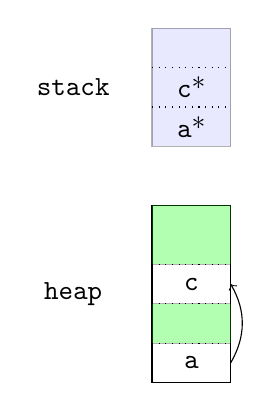
\begin{tikzpicture}
        \draw (0, 0) rectangle (1, 2.25);
        \draw[fill=green, opacity=0.3] (0, 1.5) rectangle (1, 2.25);
        \draw[fill=green, opacity=0.3] (0, 0.5) rectangle (1, 1);
        
        \draw[dotted] (0, 0.5) -- (1, 0.5);
        \node at (0.5, 0.25) {\texttt{a}};

        \draw[dotted] (0, 1) -- (1, 1);
        
        \draw[dotted] (0, 1.5) -- (1, 1.5);
        \node at (0.5, 1.25) {\texttt{c}};

        \draw (1, 0.25) edge[->, bend right] (1, 1.25);

        \draw[fill=blue!30, opacity=0.3] (0, 3) rectangle (1, 4.5);

        \draw[dotted] (0, 3.5) -- (1, 3.5);
        \node at (0.5, 3.25) {\texttt{a}*};
        
        \draw[dotted] (0, 4) -- (1, 4);
        \node at (0.5, 3.75) {\texttt{c}*};

        \node at (-1, 1.125) {\texttt{heap}};
        \node at (-1, 3.75) {\texttt{stack}};
    \end{tikzpicture}
\end{figure}
\noindent Now, we have free space at the place where \texttt{b} was being stored.

If a PL has no deallocator, the heap manager must be able to find and destroy any unreachable heap variables automatically. This is done by a garbage collector. A garbage collector must visit all the reachable heap variables. This is time consuming. 

A mark-sweep garbage collector marks all reachable heap variables, then deallocates all unmarked heap variables. The algorithm below marks all heap variables reachable from pointer $p$.
\begin{itemize}
    \item Let heap variable $v$ be the referent of $p$.
    \item If $v$ is unmarked:
    \begin{itemize}
        \item Mark $v$.
        \item For each pointer $q$ in $v$:
        \begin{itemize}
            \item Mark all heap variables reachable from $q$.
        \end{itemize}
    \end{itemize}
\end{itemize}
This is a depth-first traversal. The following is the algorithm to collect garbage.
\begin{itemize}
    \item For each pointer $p$ in a global/local variable, mark all heap variables reachable from $p$.
    \item For each heap variable $v$:
    \begin{itemize}
        \item If $v$ is unmarked, destroy $v$.
        \item Else if $v$ is marked, unmark $v$.
    \end{itemize}
\end{itemize}

We illustrate this algorithm with an example. Assume that we start with the following state of local and heap variables.
\begin{figure}[H]
    \centering
    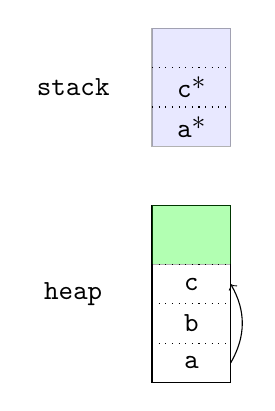
\begin{tikzpicture}
        \draw (0, 0) rectangle (1, 2.25);
        \draw[fill=green, opacity=0.3] (0, 1.5) rectangle (1, 2.25);
        
        \draw[dotted] (0, 0.5) -- (1, 0.5);
        \node at (0.5, 0.25) {\texttt{a}};

        \draw[dotted] (0, 1) -- (1, 1);
        \node at (0.5, 0.75) {\texttt{b}};
        
        \draw[dotted] (0, 1.5) -- (1, 1.5);
        \node at (0.5, 1.25) {\texttt{c}};

        \draw (1, 0.25) edge[->, bend right] (1, 1.25);

        \draw[fill=blue!30, opacity=0.3] (0, 3) rectangle (1, 4.5);

        \draw[dotted] (0, 3.5) -- (1, 3.5);
        \node at (0.5, 3.25) {\texttt{a}*};
        
        \draw[dotted] (0, 4) -- (1, 4);
        \node at (0.5, 3.75) {\texttt{c}*};

        \node at (-1, 1.125) {\texttt{heap}};
        \node at (-1, 3.75) {\texttt{stack}};
    \end{tikzpicture}
\end{figure}
\noindent We first mark all heap variables reachable from \texttt{c}.
\begin{figure}[H]
    \centering
    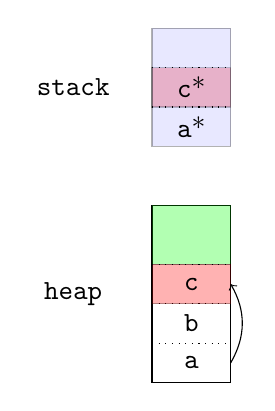
\begin{tikzpicture}
        \draw (0, 0) rectangle (1, 2.25);
        \draw[fill=green, opacity=0.3] (0, 1.5) rectangle (1, 2.25);
        \draw[fill=red, opacity=0.3] (0, 3.5) rectangle (1, 4);
        
        \draw[dotted] (0, 0.5) -- (1, 0.5);
        \node at (0.5, 0.25) {\texttt{a}};

        \draw[dotted] (0, 1) -- (1, 1);
        \node at (0.5, 0.75) {\texttt{b}};
        
        \draw[fill=red, opacity=0.3] (0, 1.5) rectangle (1, 1);
        \draw[dotted] (0, 1.5) -- (1, 1.5);
        \node at (0.5, 1.25) {\texttt{c}};

        \draw (1, 0.25) edge[->, bend right] (1, 1.25);

        \draw[fill=blue!30, opacity=0.3] (0, 3) rectangle (1, 4.5);

        \draw[dotted] (0, 3.5) -- (1, 3.5);
        \node at (0.5, 3.25) {\texttt{a}*};
        
        \draw[dotted] (0, 4) -- (1, 4);
        \node at (0.5, 3.75) {\texttt{c}*};

        \node at (-1, 1.125) {\texttt{heap}};
        \node at (-1, 3.75) {\texttt{stack}};
    \end{tikzpicture}
\end{figure}
\noindent Next, we mark all heap variables reachable from \texttt{a}.
\begin{figure}[H]
    \centering
    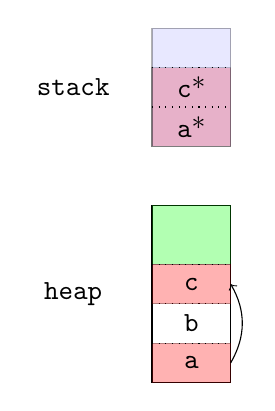
\begin{tikzpicture}
        \draw (0, 0) rectangle (1, 2.25);
        \draw[fill=green, opacity=0.3] (0, 1.5) rectangle (1, 2.25);
        \draw[fill=red, opacity=0.3] (0, 3) rectangle (1, 4);
        
        \draw[fill=red, opacity=0.3] (0, 0) rectangle (1, 0.5);
        \draw[dotted] (0, 0.5) -- (1, 0.5);
        \node at (0.5, 0.25) {\texttt{a}};

        \draw[dotted] (0, 1) -- (1, 1);
        \node at (0.5, 0.75) {\texttt{b}};
        
        \draw[fill=red, opacity=0.3] (0, 1.5) rectangle (1, 1);
        \draw[dotted] (0, 1.5) -- (1, 1.5);
        \node at (0.5, 1.25) {\texttt{c}};

        \draw (1, 0.25) edge[->, bend right] (1, 1.25);

        \draw[fill=blue!30, opacity=0.3] (0, 3) rectangle (1, 4.5);

        \draw[dotted] (0, 3.5) -- (1, 3.5);
        \node at (0.5, 3.25) {\texttt{a}*};
        
        \draw[dotted] (0, 4) -- (1, 4);
        \node at (0.5, 3.75) {\texttt{c}*};

        \node at (-1, 1.125) {\texttt{heap}};
        \node at (-1, 3.75) {\texttt{stack}};
    \end{tikzpicture}
\end{figure}
\noindent Since we only have pointers to \texttt{a} and \texttt{c} available as local variables, the marking phase is over. Now, we deallocate any unmarked variables and unmark the others.
\begin{figure}[H]
    \centering
    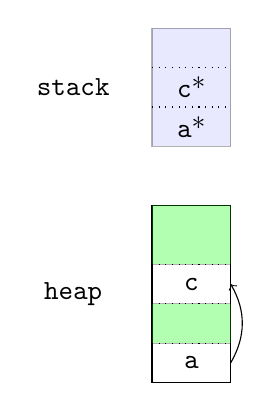
\begin{tikzpicture}
        \draw (0, 0) rectangle (1, 2.25);
        \draw[fill=green, opacity=0.3] (0, 1.5) rectangle (1, 2.25);
        \draw[fill=green, opacity=0.3] (0, 0.5) rectangle (1, 1);
        
        \draw[dotted] (0, 0.5) -- (1, 0.5);
        \node at (0.5, 0.25) {\texttt{a}};

        \draw[dotted] (0, 1) -- (1, 1);
        
        \draw[dotted] (0, 1.5) -- (1, 1.5);
        \node at (0.5, 1.25) {\texttt{c}};

        \draw (1, 0.25) edge[->, bend right] (1, 1.25);

        \draw[fill=blue!30, opacity=0.3] (0, 3) rectangle (1, 4.5);

        \draw[dotted] (0, 3.5) -- (1, 3.5);
        \node at (0.5, 3.25) {\texttt{a}*};
        
        \draw[dotted] (0, 4) -- (1, 4);
        \node at (0.5, 3.75) {\texttt{c}*};

        \node at (-1, 1.125) {\texttt{heap}};
        \node at (-1, 3.75) {\texttt{stack}};
    \end{tikzpicture}
\end{figure}

The time complexity of mark-sweep garbage collection is $O(n_r + n_h)$, where $n_r$ is the number of reachable heap variables and $n_h$ the number of heap variables. Moreover, the heap tends to become fragmented. There might be many small areas, but none big enough to allocate a new large heap variable. We could mitigate this by coalescing adjacent free areas in the heap. A better solution, however, is to use a copying or generational garbage collector.

A copying garable collector maintains two separate heap spaces. Initially, space 1 contains all heap variables and space 2 is spare. Whenever the garable collector reaches a marked heap variable $v$, it copies $v$ from space 1 to space 2. At the end of garbage collection, spaces 1 and 2 are swapped. This way, heap variables can be consolidated when copied into space 2. However, all pointers to a copied heap variable must be found and redirected from space 1 to space 2.

A generational garbage collector maintains two (or more) separate heap spaces. One space (the old generation) contains only long-lived heap variables. The other space (the young generation) contains shorter-lived heap variables. The old generation is garbage-collected infrequently, while the young generation is garbage-collected frequently. Heap variables that live long enough may be promoted from the young generation to the old generation. We can use different strategies for garbage collection depending on the generation. This technique allows for a more focused garbage collection, and is used by many PLs. 

\newpage

\section{Native code generation}
Code selection is difficult for real machines because CISC (complex instruction set computer) machines have very complicated instructions with multiple addressing modes. Even RISC (reduced instruction set computer) machines have fairly complicated instructions.

Register allocation for real machines is an issue. Registers should be used as much as possible. RISC machines typically have only general-purpose registers. CISC machines typically have a variety of special-purpose registers (e.g. int registers, float registers and address registers).

Registers are fast. So, we aim to use registers as much as possible for local variables and intermediate results of expressions. The issue is that the number of registers is limited. Different variables can be allocated the same register if their lifetimes do not overlap. Hwere, a variable is deemed to be live only if it might be inspected later.

A basic block (BB) is a stright-line sequence of instructions. There are no jumps expect at the end of the BB. Moreover, there are no jumps to anywhere expect the start of a BB. Within a BB, we break up complicated expressions using temporary variables such that each assignment instruction contains at most one operator. 

For example, if we have the operation \texttt{a = (b + c) * (d - e)}, then we can store \texttt{b + c} and \texttt{d - e} in temporary variables, and then compute the result. The sequence of 3 instructions- computing the sum, the difference and the final product is a BB.
The actual BB code is the following.
\begin{lstlisting}
t1 <- b + c
t2 <- d - e
a <- t1 x t2
\end{lstlisting}

Consider the following C function.
\begin{lstlisting}[language=C]
int tri(int a, int b, int c) {
    int s = (a + b + c)/2;
    return s * (s - a) * (s - b) * (s - c);
}
\end{lstlisting}
The function is a single BB, as shown below.
\begin{lstlisting}
t1 <- a + b
t2 <- t1 + c
s <- t2 / 2
t3 <- s - a
t4 <- s x t3
t5 <- s - b
t6 <- t4 x t5
t7 <- s - c
t8 <- t6 x t7
return t8
\end{lstlisting}

Within the BB, we determine where each variable is alive and then allocate registers.
\begin{figure}[H]
    \centering
    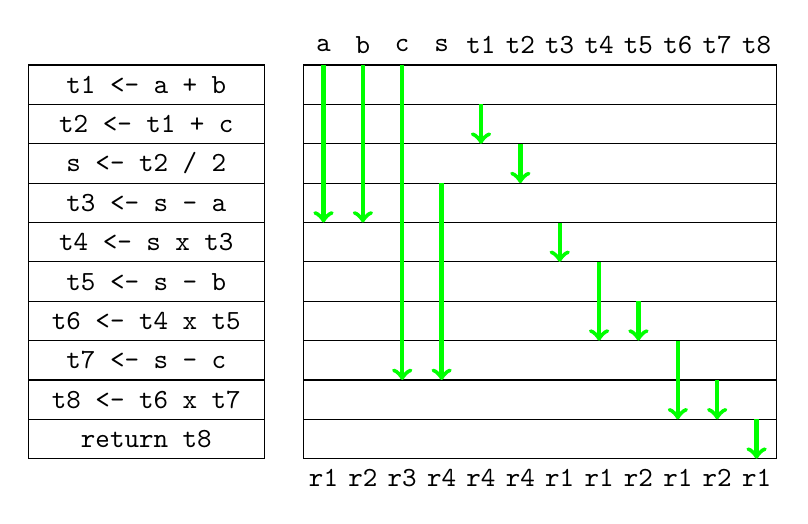
\begin{tikzpicture}
        \foreach \code[count=\i] in {
            t1 <- a + b,
            t2 <- t1 + c,
            s <- t2 / 2,
            t3 <- s - a,
            t4 <- s x t3,
            t5 <- s - b,
            t6 <- t4 x t5,
            t7 <- s - c,
            t8 <- t6 x t7,
            return t8} 
        {
            \node at (-2, -0.5*\i) {\texttt{\code}};
            \draw (-3.5, -0.5*\i-0.25) rectangle (-0.5, -0.5*\i+0.25);
            \draw (0, -0.5*\i-0.25) rectangle (6, -0.5*\i+0.25);
        }

        \foreach \x[count=\i] in {a, b, c, s, t1, t2, t3, t4, t5, t6, t7, t8} {
            \node at (\i*0.5-0.25, 0) {\texttt{\x}};
        }
        
        \draw[->, ultra thick, green] (0.25, -0.25) -- (0.25, -2.25);
        \draw[->, ultra thick, green] (0.75, -0.25) -- (0.75, -2.25);
        \draw[->, ultra thick, green] (1.25, -0.25) -- (1.25, -4.25);
        \draw[->, ultra thick, green] (1.75, -1.75) -- (1.75, -4.25);
        \draw[->, ultra thick, green] (2.25, -0.75) -- (2.25, -1.25);
        \draw[->, ultra thick, green] (2.75, -1.25) -- (2.75, -1.75);
        \draw[->, ultra thick, green] (3.25, -2.25) -- (3.25, -2.75);
        \draw[->, ultra thick, green] (3.75, -2.75) -- (3.75, -3.75);
        \draw[->, ultra thick, green] (4.25, -3.25) -- (4.25, -3.75);
        \draw[->, ultra thick, green] (4.75, -3.75) -- (4.75, -4.75);
        \draw[->, ultra thick, green] (5.25, -4.25) -- (5.25, -4.75);
        \draw[->, ultra thick, green] (5.75, -4.75) -- (5.75, -5.25);
        
        \foreach \x[count=\i] in {r1, r2, r3, r4, r4, r4, r1, r1, r2, r1, r2, r1} {
            \node at (\i*0.5-0.25, -5.5) {\texttt{\x}};
        }
    \end{tikzpicture}
\end{figure}

A control-flow graph is a directed graph in which:
\begin{itemize}
    \item each vertex is a BB;
    \item each edge is a jump from the end of one BB to the start of another BB;
    \item one vertex is designated as the entry point; and
    \item one vertex is designated as the exit point.
\end{itemize}
Consider the following C program:
\begin{lstlisting}[language=C]
int pow(int b, int n) {
    int p = 1;
    int q = b;
    int m = n;
    while (m > 0) {
        if (m & 1) {
            p = p * q;
        }
        m = m / 2;
        q = q * q;
    }
    return p;
}
\end{lstlisting}
Its control-flow graph is given below.

Each section is a BB. We consider which variables are alive at BB.
\begin{itemize}
    \item $b$ and $n$ are alive only in BB1;
    \item $p$ is alive everywhere;
    \item $m$ and $q$ are alive everywhere except in BB6;
    \item $t1$ is alive only in BB2; and
    \item $t2$ is alive only in BB3.
\end{itemize}

For each BB $b$, we define the following 4 sets of variables in a control-flow graph:
\begin{itemize}
    \item in[b] is the set of variables that are alive at the start of $b$;
    \item out[b] is the set of variables that are alive at the end of $b$;
    \item use[b] is the set of variables $v$ such that $b$ inspects $v$ (before any update to $v$);
    \item def[b] is the set of variables $v$ such that $b$ updates $v$ (before any inspection of $v$).
\end{itemize}
We have
\[in[b] = use[b] \cup (out[b] - def[b]),\]
and
\[out[b] = in[b'] \cup in[b''] \cup \dots,\]
where $b'$, $b''$ are the successors of $b$ in the flow graph.

Theseq equations give rise to the liveness analysis algorithm. We compute in[b] and out[b] for all BBs in a control flow graph.
\begin{itemize}
    \item For each $b$:
    \begin{itemize}
        \item Set $in[b] = out[b] = \{\}$.
    \end{itemize}
    \item Repeat until the sets $in[b]$ and $out[b]$ stop changing.
    \begin{itemize}
        \item For each $b$:
        \begin{enumerate}
            \item Set $in[b] = use[b] \cup (out[b] - def[b])$.
            \item Set $out[b] = in[b'] \cup in[b''] \cup \dots$, where $b'$, $b''$, $\dots$ are the successors of $b$.
        \end{enumerate}
    \end{itemize}
\end{itemize}
The live variables in block $b$ are $in[b] \cup def[b]$.

We illustrate this with an example. We have 
\begin{align*}
    use[BB1] &= \{b, n\} & def[BB1] &= \{p, q, m\} \\
    use[BB2] &= \{m\} & def[BB2] &= \{t1\} \\
    use[BB3] &= \{m\} & def[BB3] &= \{t2\} \\
    use[BB4] &= \{p, q\} & def[BB4] &= \{\} \\
    use[BB5] &= \{m, q\} & def[BB5] &= \{\} \\
    use[BB6] &= \{p\} & def[BB6] &= \{\}
\end{align*}
Next, we compute in and out.
\begin{align*}
    in[BB1] &= \{b, n\} \cup (out[BB1] - \{p, q, m\}) & out[BB1] &= in[BB2] \\
    in[BB2] &= \{m\} \cup (out[BB2] - \{t1\}) & out[BB2] &= in[BB6] \cup in[BB3] \\
    in[BB3] &= \{m\} \cup (out[BB3] - \{t2\}) & out[BB3] &= in[BB5] \cup in[BB4] \\
    in[BB4] &= \{p, q\} \cup out[BB4] & out[BB4] &= in[BB5] \\
    in[BB5] &= \{m, q\} \cup out[BB5] & out[BB5] &= in[BB2] \\
    in[BB6] &= \{p\} \cup out[BB6] & out[BB6] &= \{\}
\end{align*}
Substituting the out variables, we get the folllowing in variables for each BB:
\begin{align*}
    in[BB1] &= \{b, n\} \cup (in[BB2] - \{p, q, m\}) \\
    in[BB2] &= \{m\} \cup ((in[BB6] \cup in[BB3]) - \{t1\}) \\
    in[BB3] &= \{m\} \cup ((in[BB5] \cup in[BB4]) - \{t2\}) \\
    in[BB4] &= \{p, q\} \cup in[BB5] \\
    in[BB5] &= \{m, q\} \cup in[BB2] \\
    in[BB6] &= \{p\}.
\end{align*}
Starting with $in[b] = \{\}$, we try to converge to a fixed point.
\begin{table}[H]
    \centering
    \begin{tabular}{|c|c|c|c|c|c|}
        \hline
        in[BB1] & in[BB2] & in[BB3] & in[BB4] & in[BB5] & in[BB6] \\
        \hline
        $\{\}$ & $\{\}$ & $\{\}$ & $\{\}$ & $\{\}$ & $\{\}$ \\
        $\{b, n\}$ & $\{m\}$ & $\{m\}$ & $\{p, q\}$ & $\{m, q\}$ & $\{p\}$ \\ 
        $\{b, n\}$ & $\{m, p\}$ & $\{m, p, q\}$ & $\{m, p, q\}$ & $\{m, p, q\}$ & $\{p\}$ \\ 
        $\{b, n\}$ & $\{m, p, q\}$ & $\{m, p, q\}$ & $\{m, p, q\}$ & $\{m, p, q\}$ & $\{p\}$ \\  
        $\{b, n\}$ & $\{m, p, q\}$ & $\{m, p, q\}$ & $\{m, p, q\}$ & $\{m, p, q\}$ & $\{p\}$ \\ 
        \hline
    \end{tabular}
\end{table}
\noindent This process terminates after 5 iterations because the set of all variables has stopped changing.

\subsection{Intermediate Representation}
Native code generation is simplified by using a low-level intermediate representation (IR) of the source program. The IR should be able to represent the sematics of both the source code and the target machine instructions. The IR should ideally be independent of the target machine.

Consider the C assignment \texttt{a[i] = v}. Assume that \texttt{a} has type \texttt{int*} and \texttt{v} has type \texttt{int}. Moreover, each \texttt{int} occupies 4 bytes. Variable \texttt{a} is located at offset $a$ within the topmost activation frame. The variable \texttt{i} is located in register r9. The variable \texttt{v} is located at the offset \texttt{v} within the topmost activation frame. Then, the address of \texttt{a[i]} is
\[\text{base address of } \texttt{a} + 4 \times \texttt{i}.\]
The following is the IR tree for the given code.
% TODO: Add figure

The IR trees are given below.
% TODO: ??

Now, we consider an example. Jouette is a hypothetical RISC machine. It has 32 general-purpose registers from r0 to r31. The register r0 is always zero. The following is its instruction set.
% TODO: Add table

The following are some syntax trees:
% TODO: Them trees

We translate the source code or AST into an IR tree. We cover the tree with IR instruction patterns. We emit code corresponding to these instruction patterns, performing register allocation along the way.

The AST for \texttt{a[i] = v} is the following.
\begin{lstlisting}
LOAD    r1, a(fp)
ADDI    r2, r0, 4
MUL     r2, r9, r2
ADD     r1, r1, r2
LOAD    r2, v(fp)
STORE   r2, 0 (r1)
\end{lstlisting}
% TODO: AST

\begin{lstlisting}
LOAD    r1, a(fp)
ADDI    r2, r0, 4
MUL     r2, r9, r2
ADD     r1, r1, r2
ADDI    r2, fp, v
COPY    (r2), (r1)
\end{lstlisting}
% TODO: AST

The code selection is the maximal much algorithm. To cover the IR tree $t$ using the patterns $ps$, we do the following:
\begin{itemize}
    \item find the largest pattern $p$ in $ps$ that covers the top of $t$.
    \item find each uncovered subtree $s$ of $t$ (from left to right).
    \begin{itemize}
        \item cover $s$ using $ps$.
        \item emit the instruction corresponding to $p$.
    \end{itemize}
\end{itemize}
The time complexity is $O(|t|)$. The emitted code is optimal in that no two adjacent patterns could be replaced by a single pattern. Moreover, the number of instructions is minimal.



    
\end{document}